
\begin{fullwidth}
The chapter contains the main results from simulations experiments at the individual scale. It provides insight on the impact of plastic allocation algorithm on individual growth and potential effects on community properties. 

The first part is dedicated to the parameter filtering and the study on individual growth in a stable environment. The second part examines response of individual root strategies to two gradients of water availability: (1) with constant influx but differences in means simulating spatial heterogeneity, (2) with shared mean influx, but contrasting rate of reduction of precipitation simulating the reduction of available resource during the growing season.
\end{fullwidth}

\chapter{Model properties and individual responses}
%%(Related to the notions cited above, like performance decomposition)
%Question I try to answer: (use of schematics ?)

%The modelling framework developed in previous chapter offers multiple options to explore the effect of phenotypic plasticity on plant growth, and later plant community dynamics. Before investigating the effects of such mechanisms on complex systems dynamics, it is important to have a deep understanding of the model behaviour at individual level. As explained in introduction, the relationship between resource and individual plant growth is the base for plant interactions, abiotic filtering and coexistence mechanisms.
%This chapter of the document focuses on the calibration and exploration of the model for isolated individuals. The results of the simulation experiments exploring diverse aspect of resource-plant growth relationship will be interpreted at individual scales, but I will also attempt to extend conclusion to higher level mechanisms.

The first part of the chapter is dedicated to the parameter filtering process, the sensitivity analysis and basic model behaviour. %Then follows the exploration of plant performance as a function of plant strategy and resources levels and dynamics.


% ##################################################################################
\section{Parametrisation and sensitivity analysis} \label{section:calibration}

Calibration, or \textemph{parametrisation}, is an essential step in the development of an agent-based model. ABMs are often characterised by multiple processes, and though parameters, at individual levels. The results of these processes (depending of parameter values) from numerous individuals combine to produce the group or community behaviour. Because there are interactions between the processes and between the agents, the overall behaviour of the group (often the subject of interest) is sensitive to these parameters. For the same reasons, an incredible variety of results could be produced with ABMs if the parameters where not chosen in order to produce sensible responses to simulated conditions. The aim of the calibration is to determine, from the \textit{a priori} knowledge of the processes and parameters, and the comparison with data, the best values for the model parameters. This step often goes along with a sensitivity analysis that determine the relative sensitivity of variables of interest to specific parameters.

Because of their nature, ABMs often model processes for which the parameters are either unknown, or hard to access (because at the individual scale). In such cases, advance calibration techniques like pattern oriented modelling\parencite{grimm_pattern-oriented_2005, hartig} can be developed. However, such method require a high number of simulations and relatively precise simulation parameters. Because the implementation in R makes the model relatively slow, and because available datasets, despite being very interesting lack information on sensitive parameters, a less robust but less expensive approach is chosen: \textemph{parameter filtering} at the individual scale. The focus of the part of this work on the individual growth, and the will for more individual-centric approach also support this choice.

 For similar reasons of computational cost, the \textemph{sensitivity analysis} is  realised \textit{a posteriori} on calibration runs.

\subsection{Method}

\paragraph{Pot data}
Pot data consists in total biomass and root shoot ration (RSR) data of 11 species grown in pots by Peterson and Billings \parencite{peterson_growth_1982}. This dataset has the advantages of being grass species grown in a described steady environment with two conditions of watering with measures of essential components of growth: biomass and RSR.

\paragraph{Pot simulation}
Simulated plant grow in square pots 9 cm wide and 12 cm deep. The soil is characterised by the following parameters: critical soil water content: $0.1 m^3.m^{-3}$, and saturation water content: $0.1 m^3.m^{-3}$. Simulation time of 111 days of 15 hours is divided between the growing phase of ... days, followed by the treatment phase when plant are water (soil saturation) either once a week or once a day. The light level and water influx are simulated with water event of ... mm and lighting of ... Watts per square meter.
Plants have default geometry parameters and reproduction is ignored and I assume plants do not stop their growth.

\paragraph{Parameter filtering process}
The whole filtering process has been implemented in \texttt{R}. Model parameters are sampled following the LHS method (from \texttt{lhs} package) within parameter ranges (described in table \ref{table:priors}) defined both thanks to the literature and constraints dictated by desired behaviours from the model. When necessary the sample is log transformed. Because of strong relationship between exchange rate parameters and cost of exchange area, exchanges rates parameters are expressed on a mass basis for sampling then transformed into an area basis for the model. To avoid extreme RSR ratios, the ratio between the mass based exchange rate parameters is limited between 0.1 and 10.

As explained in previous chapter, species specific parameters are requited to model plant growth. These parameters are sampled at the same time that the parameters of the model, according to ranges detailed in table \ref{table:state_var_species}.

Once the parameters generated, a first filtering is applied to save simulation time and avoid unrealistic trait values. Compute initial trait values considered out of range (see table for ranges extracted from LES data \parencite{wright_worldwide_2004} in alpine biome) are excluded.

These two steps lead to the creation of a list of $n$ independent parameter sets that are then used for individual pot simulations following Peterson and Billings experiment sett-up.

Results from finished simulations (i.e. plant lives until the end and do not exceed model's internal size limits) are then compared to experiment data species by species. Parameters of logistic distribution are computed from species means and standards deviations for RSR and total biomass. The use of this distribution form is justified by the intrinsic form of RSR measure and the need to reject negative values for total biomass. A parameter set is accepted for one species if it within a 95\% range of the calculated distribution for both RSR and total biomass in wet and dry conditions.

The parameter filtering procedure is applied on the three main allocation algorithms: \textit{non plastic}, \textit{fixed-equilibrium} and \textit{plastic-optimisation}.

\begin{figure}\label{fig:comparison_BM}
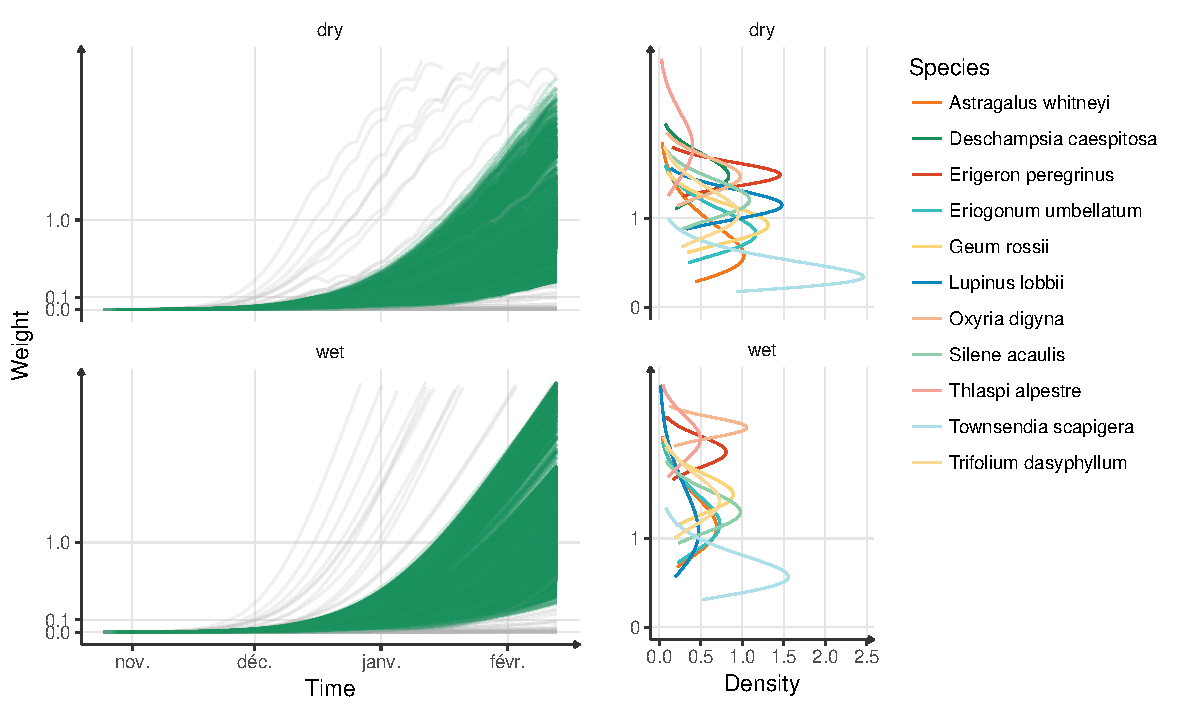
\includegraphics[width = \textwidth]{./2_PP/Figures/Calibration/weight_full_sim.pdf}
\caption{Comparison of simulated weights with distribution of weights of real alpine species for contrasting conditions.}
\end{figure}

\paragraph{Sensitivity analysis}
Relative importance of variables in the selection process is investigated with the packages \texttt{randomForest}. A random forest analysis (depth = 5, number of trees = 300) is performed on a balance dataset composed by all selected parameter sets and a random sample of rejected sets of equal size. Importance is assessed on the results of the random forest.

\subsection{Results}

\paragraph{Selection rate}
Parameter filtering process resulted in the selection of a low number of parameter sets (below 0.2\%) for each allocation algorithms (table \ref{table:selection_rate}). This number is below the sum of accepted parameter sets per species because a parameter set can match to multiple species. Not all species contribute to the same extend to the filtering process. \textit{Astragalus whitneyi} accounts for a high percentage of accepted parameter sets, while no parameter set could match 2 species (\textit{Oxyria dignya} and \textit{Deschampsia caespitosa}). The former is characterised by wide distribution in both conditions for the two variables of interest (weight and RSR), while the latter show relatively tight distribution with little overlap between the conditions for the both variables (see figure \ref{fig:comparison_BM} for comparison between simulations and data for total weight).

% latex table generated in R 3.2.3 by xtable 1.8-2 package
% Wed Nov 15 13:39:16 2017
\begin{table2*}\label{table:selection_rate}
\caption{Acceptance rate per species for the 3 main allocation algorithms. Because some parameter sets match multiple species, the total number and rate of accepted parameter sets is lower than the sum of accepted parameter sets per species. All rates are given in \%. }
%\centering
\begin{tabular}{lrr|rr|rr}
 & & non plastic & & fixed-eq & & plastic \\
  \hline
 species & n (2M) & rate & n (2M) & rate & n (200,000) & rate \\
% species & n (995603) & rate (\%) & n (995539) & rate & n (199964) & rate \\ 
  \hline
 Silene acaulis & 227 & 0.02 & 396 & 0.04 & 55 & 0.03 \\ 
 Trifolium dasyphyllum & 271 & 0.03 &  317 & 0.03 & 45 & 0.02\\ 
 Geum rossii & 51 & 0.01 & 72 & 0.01 & 12 & 0.01\\ 
 Thlaspi alpestre & 342 & 0.03 & 360 & 0.04 & 59 & 0.03\\ 
 Deschampsia caespitosa & - & - & - & - & - & -\\ 
 Eriogonum umbellatum & 500 & 0.05 & 805 & 0.08 & 118 & 0.06\\ 
 Townsendia scapigera & 593 & 0.06 & 930 & 0.09 & 107 & 0.05\\ 
 Astragalus whitneyi & 1570 & 0.016 & 2424 & 0.24 & 318 & 0.16\\ 
 Lupinus lobbii & 678 & 0.07 &  868 & 0.09 & 123 & 0.06\\ 
 Erigeron peregrinus & 1 & <0.01 & - & - & - \\ 
 Oxyria digyna & - & - & - & - & - & - \\ 
  \hline
  Total & 4233 & 0.43 & 6172 & 0.62 & 837 & 0.42\\
  \hline
 \textbf{Accepted} & 924 & 0.\textbf{09} & 1416 & \textbf{0.14} & 200 & \textbf{0.10}\\
\end{tabular}\end{table2*}

Despite the low selection rate, a difference can be noted between the \textit{fixed-equilibrium} algorithm and the two other algorithms with a accepted rate of 0.14 \% against 0.09\% and 0.10\% (table \ref{table:selection_rate}). This difference cannot be explained by a significantly better selection rate for specific species, but rather higher rates for all species.

Most of parameter sets are not shared between the algorithms (\textit{i.e.} around respectively and third and a quarter of accepted parameter sets are shared between \textit{non plastic} allocation and \textit{fixed-equilibrium} allocation calibrations), despite that the distribution of parameter values that are not shared are very similar and do not show any clear pattern (data not shown).

Out of the 31 parameters, 6 show graphical response of selection rate (see figure \ref{fig:accept_rate}), and only  \texttt{u\_max} and \texttt{P\_max} present a possible optimum different from limit values. The relative importance of the parameters is better explored in sensitivity analysis.



%Calibration filtering results in the selection of n parameter sets over m preselected parameters sets. Accepted sets are distributed among the 11 species of the dataset like presented in the table. Species A, B and C are the most numerous.\\


%Plasticity does not change the acceptance rate in any form (only slight increased from 0.26\% to 0.38\%, up to 0.42\% for full plastic). \\


\begin{figure}[p]\label{fig:accept_rate}
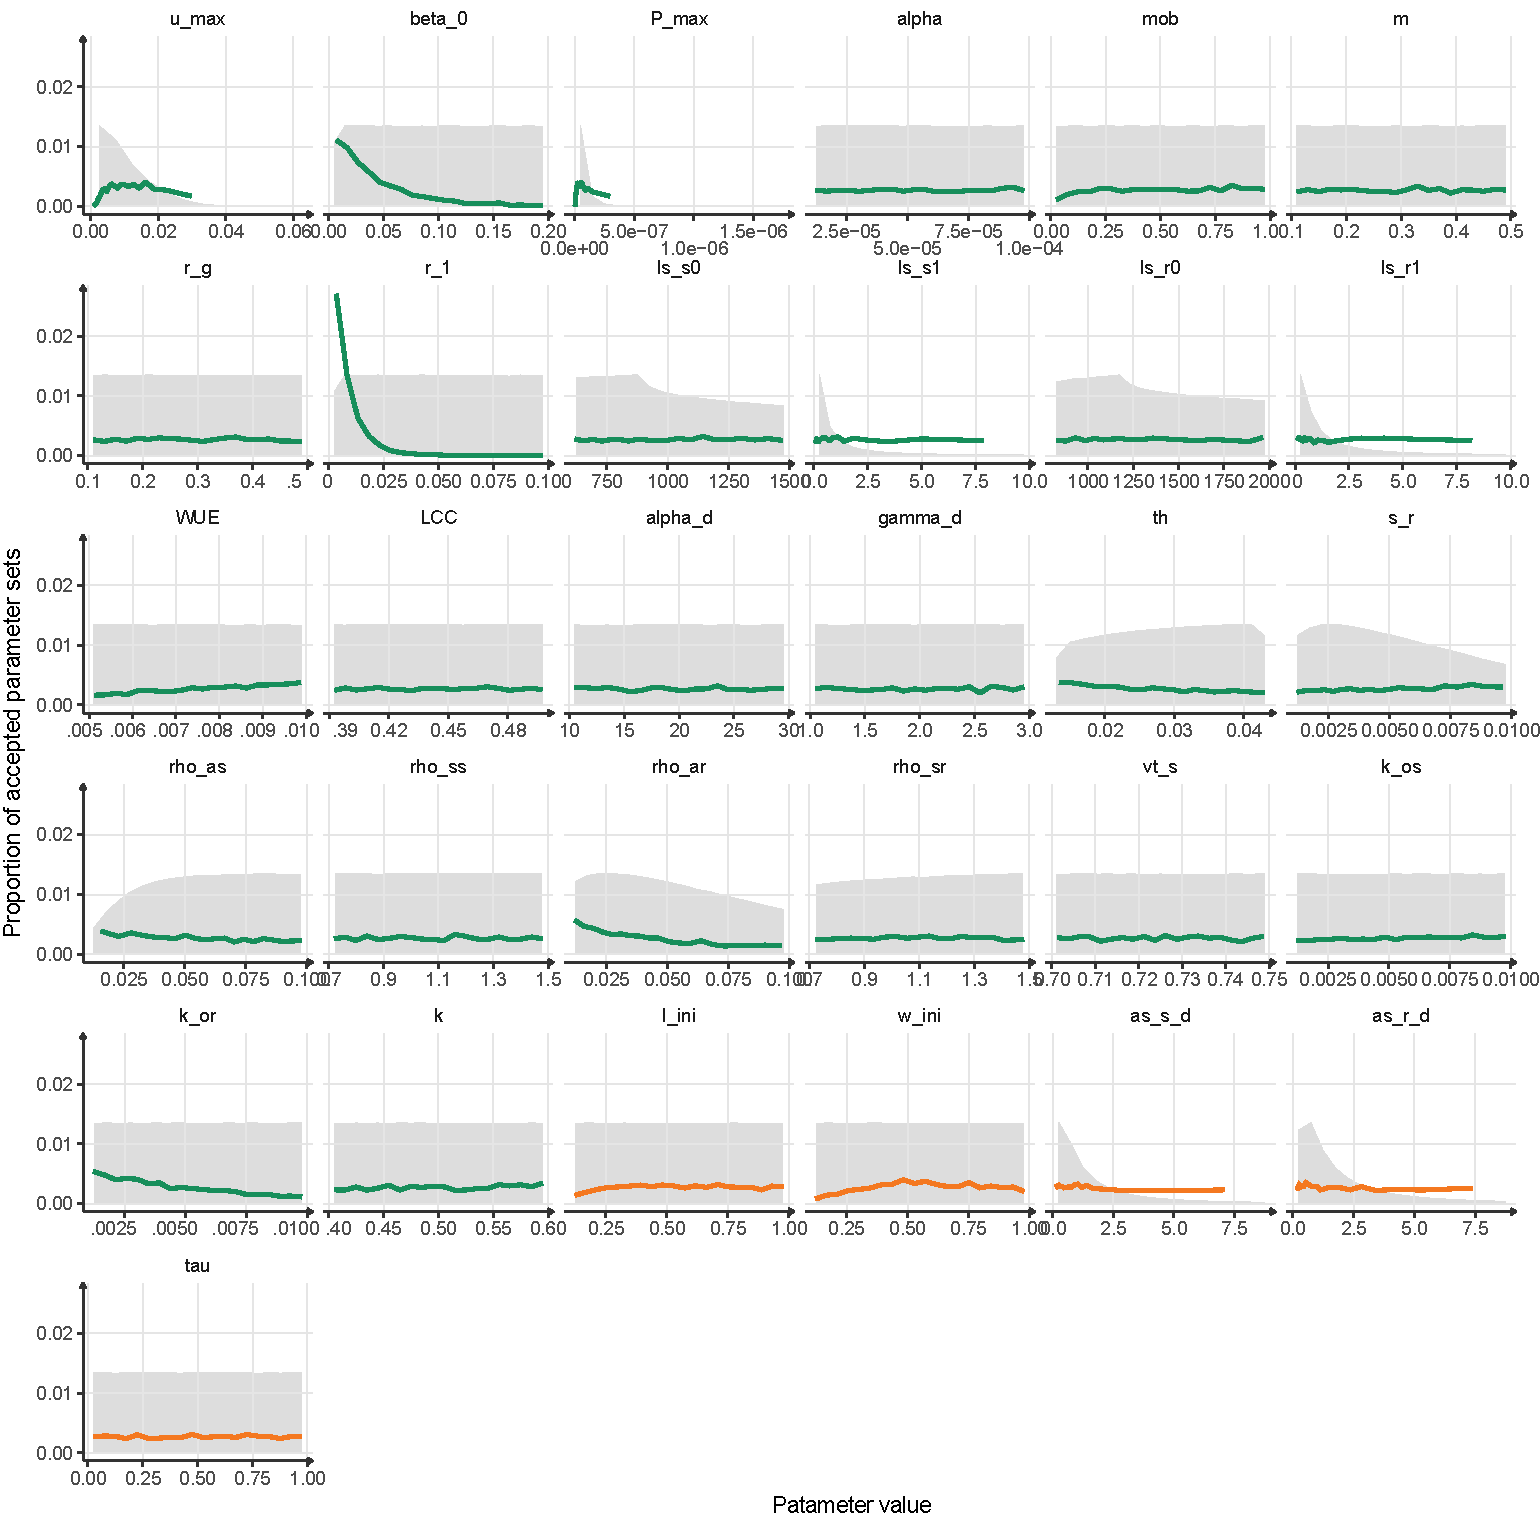
\includegraphics[width = \textwidth]{./2_PP/Figures/Calibration/acceptance_rate_RSRnWeight_per_par_none.pdf}
\caption{Selection rate per parameter for individual growth. \textit{Non plastic}.}
\end{figure}


%\begin{figure}
%%\includegraphics[width = 10cm]{/mnt/quadri1/simulations/exploration/species_par_space2017-11-06/plots/var_imp_plot_eq_design.pdf}
%\caption{Importance of the random forest to explain filtering outcome (accepted or rejected) of a balanced sample of parameter set between all tested (all accepted parameters and an equivalent sample in rejected parameters).  Fixed-equilibrium.}
%\end{figure}

\paragraph{Sensitivity analysis}


A total of 12 parameters show relative influence on selection rate for at least one of the algorithm. These parameters are divided between model parameters and species parameters. Species parameters show influence only for the \textit{non plastic}allocation algorithm. Model parameters express relatively similar importance for all three algorithms. The respiration rate of active tissues (\texttt{r\_1}) is the most sensitive parameters (see figures \ref{fig:accept_rate} and \ref{fig:importance}). Other sensitive parameters are related to water availability (\texttt{beta\_0}), organ exchange rates (\texttt{P\_max} and \texttt{u\_max}) and soil coverage by roots (\texttt{rho\_ ar} and \texttt{k\_or}).

\begin{marginfigure}\label{fig:importance}
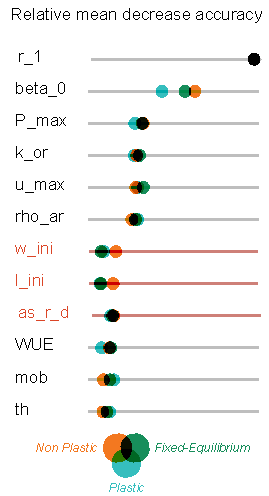
\includegraphics[width = \textwidth]{./2_PP/Figures/Calibration/importance.pdf}
\caption[Relative importance of main parameters for selection]{Relative importance of main parameters for selection under the three main allocation algorithms: (\textcolor{myOrange}{non plastic}, \textcolor{myGreen}{fixed-equilibrium} \& \textcolor{myBlue}{plastic}).}
\end{marginfigure}


%\begin{figure}[!h]
%   \begin{floatrow}
%\ffigbox{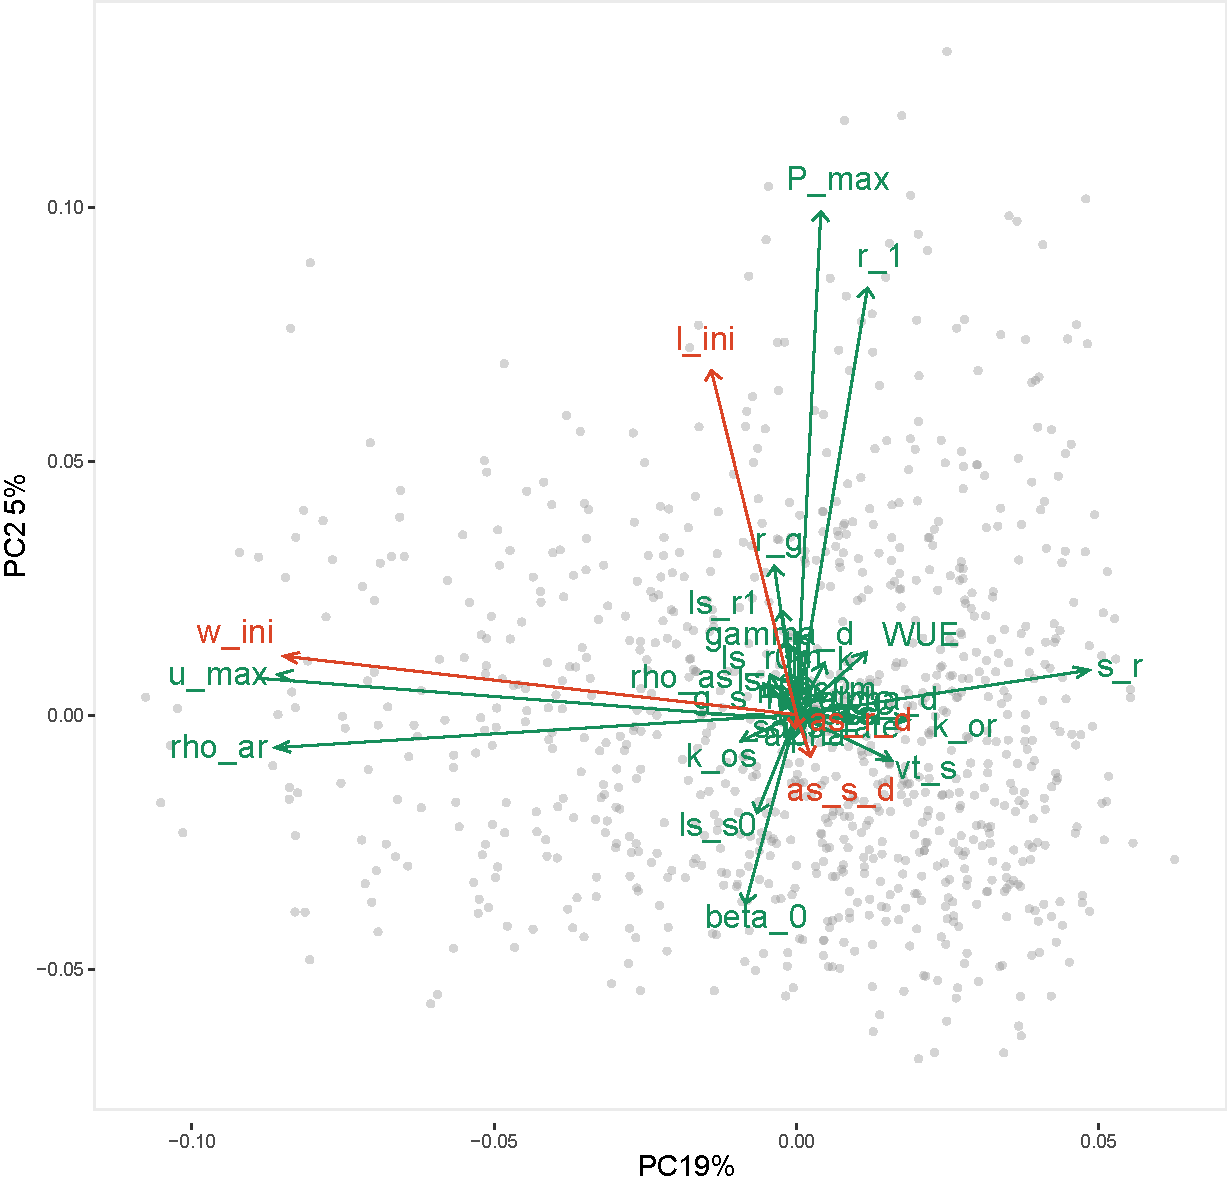
\includegraphics[width=\linewidth]{./2_PP/Figures/Calibration/PCA_none.pdf}}%
%\caption{First two axis of PCA of parameter sets selected in parameter filtering process. \textit{Non plastic}.}\label{fig:PCA_calibration}
%%       {\caption{second figure}\label{fig:example-2}}
%   \end{floatrow}
%\end{figure}
%\lipsum[3]

\begin{figure}%[tb]
    \classiccaptionstyle
\sidebysidecaption{0.60\textwidth}{0.3\textwidth}{%
    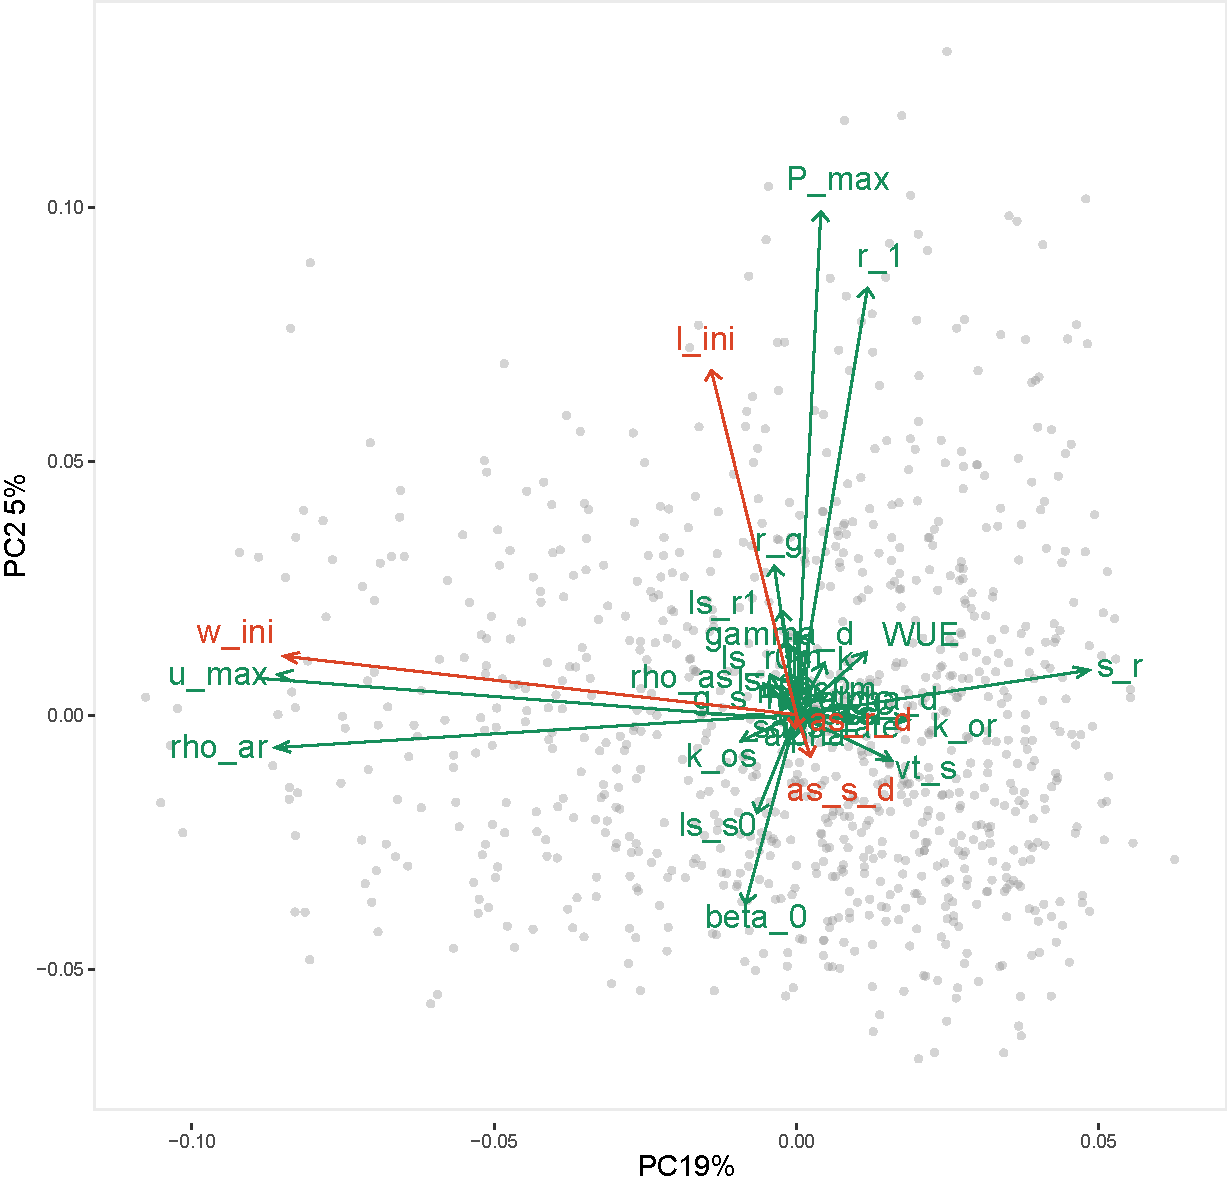
\includegraphics[width=1\linewidth]{./2_PP/Figures/Calibration/PCA_none.pdf}%
}{%
  \caption[PCA calibration]{Representation of the PCA of parameter sets selected in parameter filtering process on the first principal components. \textit{Non plastic}.}
  \label{fg:PCA_calibration}
  }
\end{figure}

The PCA performed for \textit{non plastic} algorithm only on parameter values reveals that important parameters are also the dominant variables that shapes the selected subspace. The two first axis explain only 14\% of variance. The first one is related to the root activity and efficiency (\texttt{u\_max}, \texttt{l\_ini}, \texttt{rho\_ar} and \texttt{s\_r}), the second is in line with global efficiency and resource availability.

The parameter filtering process is based on individual species, ... Species cannot be distinguished on these two main component space, neither on species specific parameters space (\texttt{l\_ini}, \texttt{w\_ini}, \texttt{w\_ini} \& \texttt{l\_ini}, \texttt{as\_s\_d}, \texttt{as\_r\_d}, \texttt{as\_r\_d} \& \texttt{as\_s\_d}) despite small variations in distribution shapes and ranges between species (data not shown).\\

\paragraph{Variable responses}
% Response of the two main vairables to main parameters.
For each algorithm the response of the two filtering variables (weight and RSR) are plotted against the most important variables in figures \ref{fig:sensitivity_BM} and \ref{ fig:sensitivity_BM}.

% Biomass
Total biomass is particularly sensitive to tissue respiration cost (\texttt{r\_1)}, but also maximum exchange rate parameters. There is a notable difference in growth maxima between the two conditions in favour of wet conditions, in line with observed data. This difference is observed for the three algorithm that differ mainly by the amplitude of the biomass ranges (need data).  Growth response curves are similar for all allocation algorithm. Growth is only weakly related to species specific parameters. Total biomass under \textit{Plastic-optimisation} algorithm seems to be more sensitive to variables influencing the exchange area per unit of biomass.

The species specific parameters \texttt{tau} controlling the balance between genetic and environmental control does not emerge as a influencing parameter at the global scale for any of the two flexible allocation rules.

\begin{figure}\label{fig:sensitivity_BM}
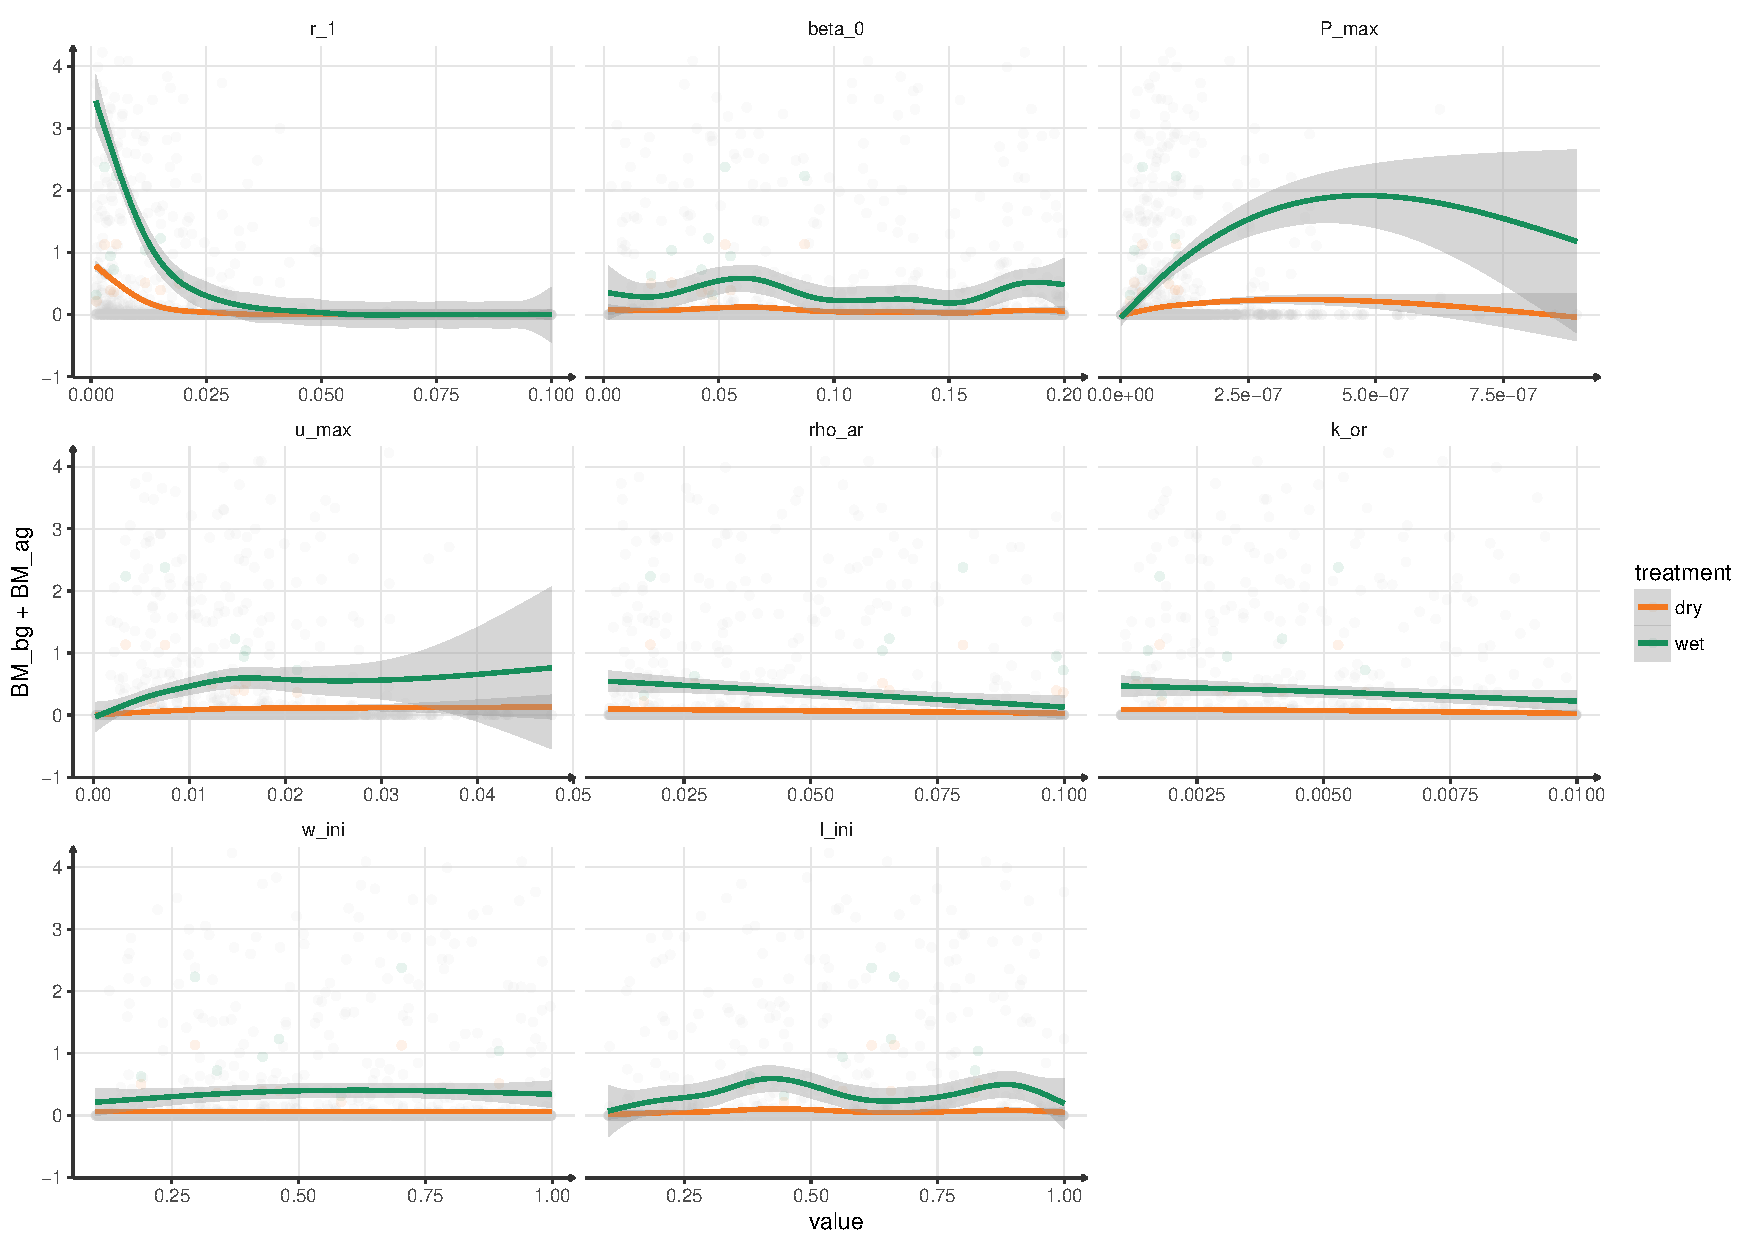
\includegraphics[width = \textwidth]{./2_PP/Figures/Calibration/par_effect_none_BM.pdf}
\caption{Main parameters effect on the total plant biomass. \textit{Non plastic}. One dot represents a parameter set. Not all parameter set are represented as the y axis is limited around the smooth function (loess). Coloured points represent selected parameter sets in the two treatments (\textcolor{myOrange}{dry} and \textcolor{myGreen}{wet}).}
\end{figure}

% RSR
Root:Shoot Ratio (or RMF in figure \ref{fig:sensitivity_RSR}) strongly responds to species specific parameters under \textit{non plastic} allocation because the memory parameters(\texttt{l\_ini} and \texttt{w\_ini}) are the means plants control their RSR. For other allocation rules, species specific parameters have little control over RSR. Surprisingly, the photosynthetic capacity has stronger influence on the ratio than the root maximum exchange rate.


\begin{figure}\label{fig:sensitivity_RSR}
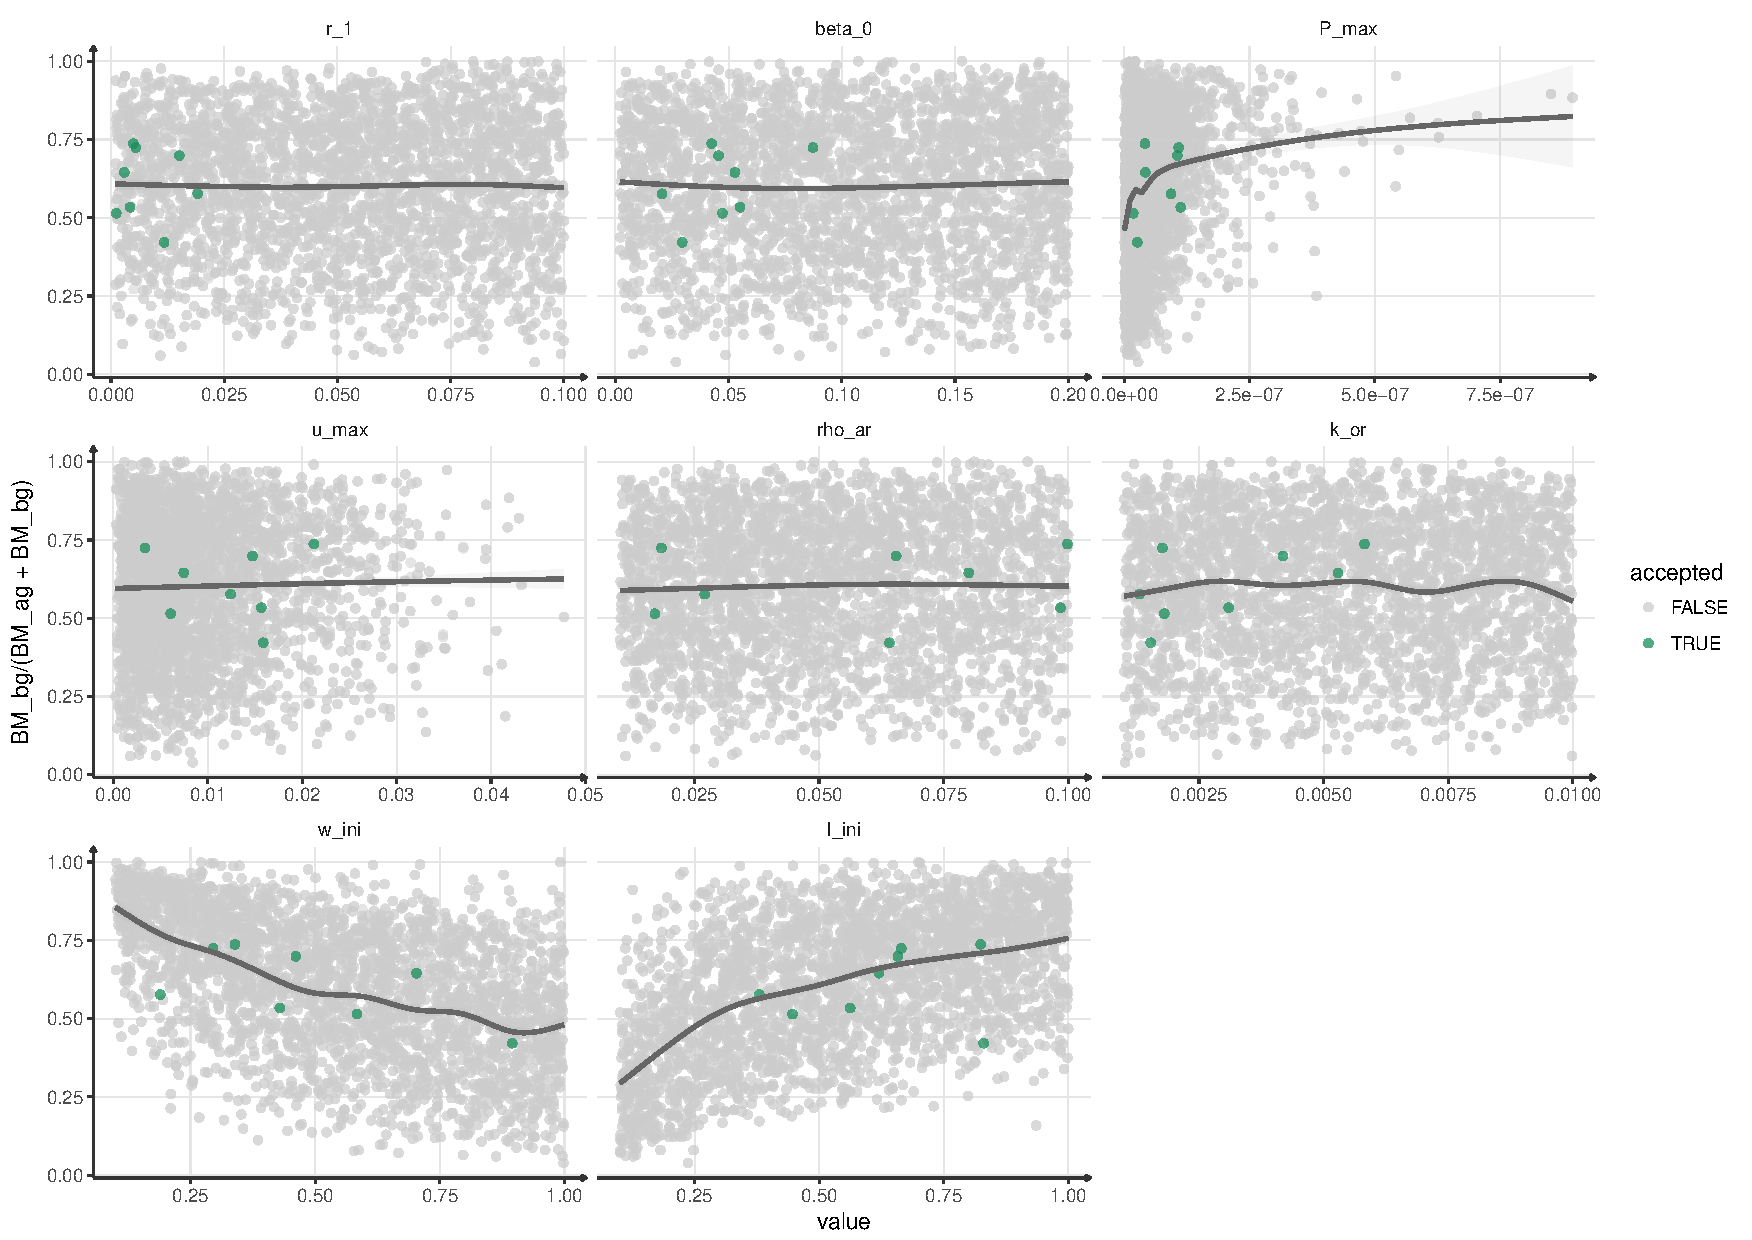
\includegraphics[width = \textwidth]{./2_PP/Figures/Calibration/par_effect_none_RSR.pdf}
\caption{Main parameters effect on the total plant Root Mass Fraction (RMF). \textit{Non plastic}}
\end{figure}

% TAU

\paragraph{Root shoot ratio and plasticity}

Little to no difference in RSR is expected for \textit{non plastic} allocation rule since allocation promoted a fixed phenotype, but both \textit{fixed-equilibrium} and \textit{plastic-optimisation} allocation rules allow for changes in RSR. Nevertheless, no stable change in RSR is observed in any of the simulations. Fluctuations are present but consist in stable oscillations between two fixed values (see figure \ref{fig:comparison_RSR}), synchronized with water variations. These rapid adaptations of the relative proportion of roots denote a high flexibility of plant phenotypes in \model.


\begin{figure}\label{fig:comparison_RSR}
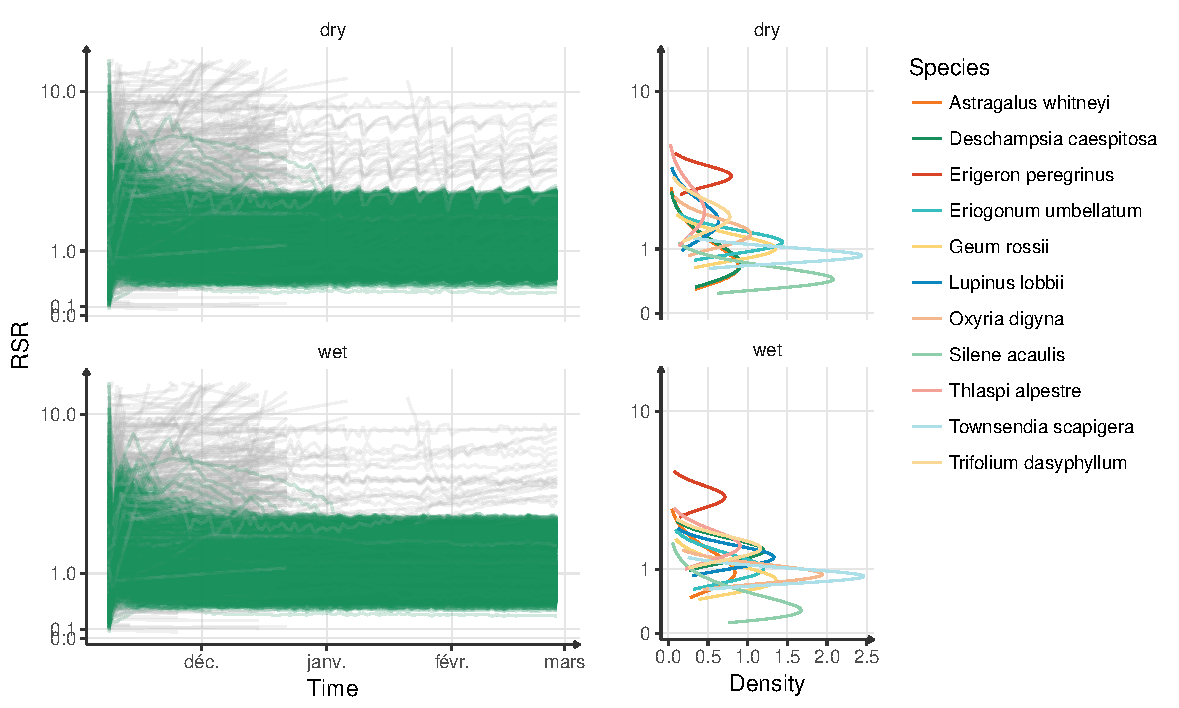
\includegraphics[width = \textwidth]{./2_PP/Figures/Calibration/RSR_full_sim_f-e.pdf}
\caption{Comparison of simulated values of RSR with real species RSR in two contrasting conditons. Because there is no plasticity or ontogeny, the simulated plant do not express any chagnes in RSR.\textit{Fixed-equilibrium}.}
\end{figure}

\subsection{Discussion}

\paragraph{Growth and strategy space}

The relative low selection rates for all allocation rules highlight the complexity of fitting such complex model to empirical data, despite the relative simplicity of the data. This difficulty seems to lie in two factors: the high number of parameters and the lack of stable changes in RSR. This last point is further discussed in the following paragraphs. Nevertheless, plant growth is reproduced in two contrasting conditions for multiple species, and while plastic algorithms have a greater potential for growth (more high growth rate), this is not systematic and the absence of clear pattern for the most influencing parameters, such as maximum exchange rates and respiration rates, indicates that such high growth depends on a combination of parameter values. I believe that the shape of gain and cost functions along the functional trade-off between active and structural tissues plays a determining role in the growth. A trade-off function with a wider viable range is more likely to be selected as more strategies would grow (therefore reducing the relative sensitivity to species-specific parameters). Considering the exponential shape of the turn-over function (one of the main cost with respiration), the width and height of the trade-off (or net gain function) is probably more strongly linked to the gain functions (exchange rates) and linear cost function (respiration), explaining little effect of parameters related to lifespan (already preselected otherwise). There is a strong dependency between viable strategies (and as a consequence functional potential diversity) and the main trade-off between resource acquisition and efficiency.

Filtering the parameter sets based on all species instead of individually would have been ideal to quantify this link and better calibrate the model. However, such approach would have required many more simulations, when the parameter filtering method was chosen for its low computational cost. Moreover, considering the number of species-specific parameters, fitting the strategy subspace (at least default active tissue allocation parameters, the memory of resources and stability) of 11 species to the data in combination with more than 20 models parameters is near impossible. Ones should have had first determined the relative positions of the species within the said strategy space before any global calibration routine. Nonetheless, species-specific parameters have an influence on model main variables. Memory parameter affected the RSR in the context of \textit{non plastic} allocation rule (see figures \ref{fig:comparison_RSR} and \ref{ fig:importance}, while the default proportion of active tissues in roots was an influencing parameter in all algorithms (figure \ref{fig:importance}, \texttt{as\_r\_d}). Therefore, they should be analyzed in further simulations within the same set of model parameters.

Change in modelling paradigm. The Bayesian paradigm where the information is contained in data and revealed by the structure of the model. Go for simulation experiment approaches where the model is used as a simulation tool and results as new data. The emerging patterns inform us on the impact of the modelled mechanisms (even if they do not totally match the data). Model as an understanding tool.\\


\textbf{Growth is reproduced, but only for one species, not full strategy space.}

\paragraph{The role of water}

If the parameter filtering step did not result in the selection of optimum values for all parameters, it provides information on the main mechanisms influence plant growth. 
Indeed, the relatively high importance of parameters related to water shows the importance of the resource on the model behaviour. Both water availability (water absorption limitation, exchange rate) and root mass and construction parameters are important to match the empirical data. Considering that the calibration relies on experiment data of drought events, it is no surprise that parameters related to water economy show strong influence on the selection rate and model behaviour. In the context where the model has been developed, water shortage is expected to an important factor in community dynamics. In this perspective, the ability of \model to reproduce the difference in productivity in both conditions, and the relative sensitivity to water related parameters is an advantage. The link between water resource, species strategy, plant performance and phenotypic plasticity is explored more in details in the following section.


%Differences between algorithms that make sense: more biomass, sensitive parameters are related to how plasticity work...

\textbf{Sensitivity of different variable to the parameters make sense and align with the two criterion of selection (that work with the independence of trade-off).}

\paragraph{More complex plasticity?}

As mentioned earlier in this discussion, the model is not able to produce any shift in RSR in different water treatment. It is not a surprise for \textit{non plastic} algorithm, but the filter was still applied on this criterion to allow the comparison with plastic algorithm and to be able to measure the improvement in selection rate. However, even plastic algorithms do not show strong enough response to water treatment in term of RSR. A strong and good (in the sense it would have matched the data) is larger in amplitude and more stable in time. Such processes generally amplify with time, \textit{i.e.} when the number of drought event increases, the response (allocation to roots) increases (relative to default phenotype). Unlike natural systems, plants in \model fluctuates between two "states", or phenotypes associates to the dry and wet conditions. The RSR post drought event is reached after the first week without water. This can be explained by two main mechanisms that are related but have contrasting implications. The quickness in response to the changing conditions is allowed by relatively high assimilation rate. If the net growth rate is controlled by the total weight condition during the filtering process, the assimilation rate is not and can be compensated with relatively high turn-over rate. Net growth rate being equal, species with higher assimilation rate will have higher phenotypic flexibility (higher fraction of biomass to invest in carbon pool of choice) than species with lower assimilation rate. This flexibility, similar to reallocation, allows changes in RSR, but not the accumulation of biomass in roots. Unfortunately, both the constant turn-over rate implemented in the model, and the selection toward "wide and high" gain functions limit control on this aspect.

Moreover, the fact that plants are more productive during periods where they may not want to invest in roots strengthen this effect. Indeed, a plant would drift to higher RSR if it was more productive when pursuing the high RSR phenotype than when pursuing the low RSR phenotype. This last point mentions the "will" of the plant, in the context of \model this target phenotype is encoded in the projection of external conditions. Because this projection is daily based by design, the accumulation of drought stress is not translated in the internal projection variables of the plant (like it can be with the accumulation of phyto-hormones \parencite{need ref}). This limitation highlights a big difference between simulated plants in \model and natural plants. While solutions to overcome this problem can easily be imagined(see equation \ref{eq:projection_alt} in \ref{subsection:submodels}), they would require more parameters and introduce more complexity to the analysis. This model provides a first approach to phenotypic plasticity in grassland models and the formulation of the projection, key element of the phenotypic plasticity, is certainly a starting point for further development. Nevertheless, the differences in response to the parameters between the three allocation rules, despite shared plant functioning, demonstrate the importance of plasticity itself. And simplification of the processes should not be a reason to not explore its effects. The fact that the parameter \texttt{tau} has a relatively small impact on selection rates alos support the need to better understand all strategic axis before focusing on the effect of projection. While there are many ways of simulating the phenotypic plasticity, the parsimony is privileged. This simple representation is enough to understand the effects of active plastic allocation in association with the other strategic differences between species.


%Exchange area per biomass and sensitivity to exchange rates : trade-off are important and structuring.

%filtering on RSR to test if plasticity improved selection of parameters, = is an essential part of platn functioning.\\
\paragraph{Modelling paradigm}
Bayesian paradigm where the information is contained in data and revealed by the structure of the model. Go for simulation experiment approaches where the model is used as a simulation tool and results as new data. The emerging patterns inform us on the impact of the modelled mechanisms (even if they do not totally match the data). Model as an understanding tool.\\
%While many ways of simulating the phenotypic plasticity can be proposed, the parsimony is privileged and this representation is enough to understand the impact of related processes shared by any representation of phenotypic plasticity is the developed framework.

\textbf{Root shoot ratio changes were not captured by the model. The structure of the plasticity mechanisms does not work with the given watering cycle. Needs to add one parameter for reactivity.}



% ##################################################################################
\section{Individual level behaviour and properties}


Calibration and sensitivity analysis give information on the main processes of plant growth, but the general effects of the allocation rules on plant growth are not fully identified. In addition, because the parameter filtering processes was limited to individual plants, and the response of species specific parameters dependent on other parameters of the model, the effects of these species specific parameters should further be investigated. The objective of this part is to set better understanding on the role of \textemph{allocation rules} and species \textemph{memory} on plant development as basis for interpretation of plasticity effects in following chapters.

The challenge of the framework presented in paragraph \ref{subsection:memory} under \textit{plastic-optimisation} is to control the phenotype with the values of the memory. The risk of this approach is to have too tight estimation function of the fitness (or driving function) and to see the convergence of all species (with different memory values) toward the same phenotype (same allocation of active and structural tissues in roots and shoot). The extend to which different species memory lead to different phenotypes under full genetic control (non influence of external conditions) is explored through simulation experiment under \textit{plastic optimisation} allocation algorithm.

%Proof of concept
\subsection{Method}


%\paragraph{Strategy diversity filtering}
%To further reduce the number of parameter sets considered, we proceeded in an additional filtering step. Because the first filtering was conduced for only one strategy over the whole 4D strategy space (l\_ini,  w\_ini, as\_s\_d, as\_r\_d) it is necessary to verify that other strategies do not lead to potential Darwinian demon. This should be limited by the choice of priors, while at the same time promoted by the selection of parameters increasing growth to counter balance potential unfitted strategies\footnote{Better do that beforehand than after... But I guess it's too late now.}.

\paragraph{Allocation algorithms}
The effect of allocation rule on phenotypic development is investigated thanks to pot simulations (see Methods in \ref{section:calibration}) of 100 days in 3 watering treatment: 2mm, 8m and 16mm per day. To avoid drift in the phenotype due to allocation algorithm (see paragraph \ref{subsection:memory} on phenotypic determination), simulations where run a first time, then rerun with default specific traits matching traits at the end of the first simulation set. All four algorithms are simulated. To reduce the number of simulations 100 parameter sets are selected randomly within the accepted parameter sets for the \textit{non plastic algorithm}.

\paragraph{Memory \& phenotype}
Memory of external conditions plays a determining role in phenotypic development under \textit{plastic-optimisation} allocation rules. The effect of the memory alone (environmental cues ignored by setting \texttt{tau} to 1) on the default emerging phenotype is explored for diverse memories (9 values on the two axis from 0.1 to 1 later scaled to the maximum area exchange rates for model parameter set considered, or 81 values) for each accepted parameter set. The effect of the memory values on the final position of plants in the phenotypic space are visualised by fitting loess curves between memory values and individual trait values.

\subsection{Results}

\paragraph{Allocation rules}
think of a "showtime" visualisation that shows how growth and traits are impacted by allocation rules and \texttt{tau}.\\

Have the proportion of tissues changing over time\\

Show the respiration, assimilation and turn-over rates.\\ 

Isn't it possible to show these along memory or active/str ratio axis ?


\begin{figure}\label{fig:plastic_allocation_trajectory}
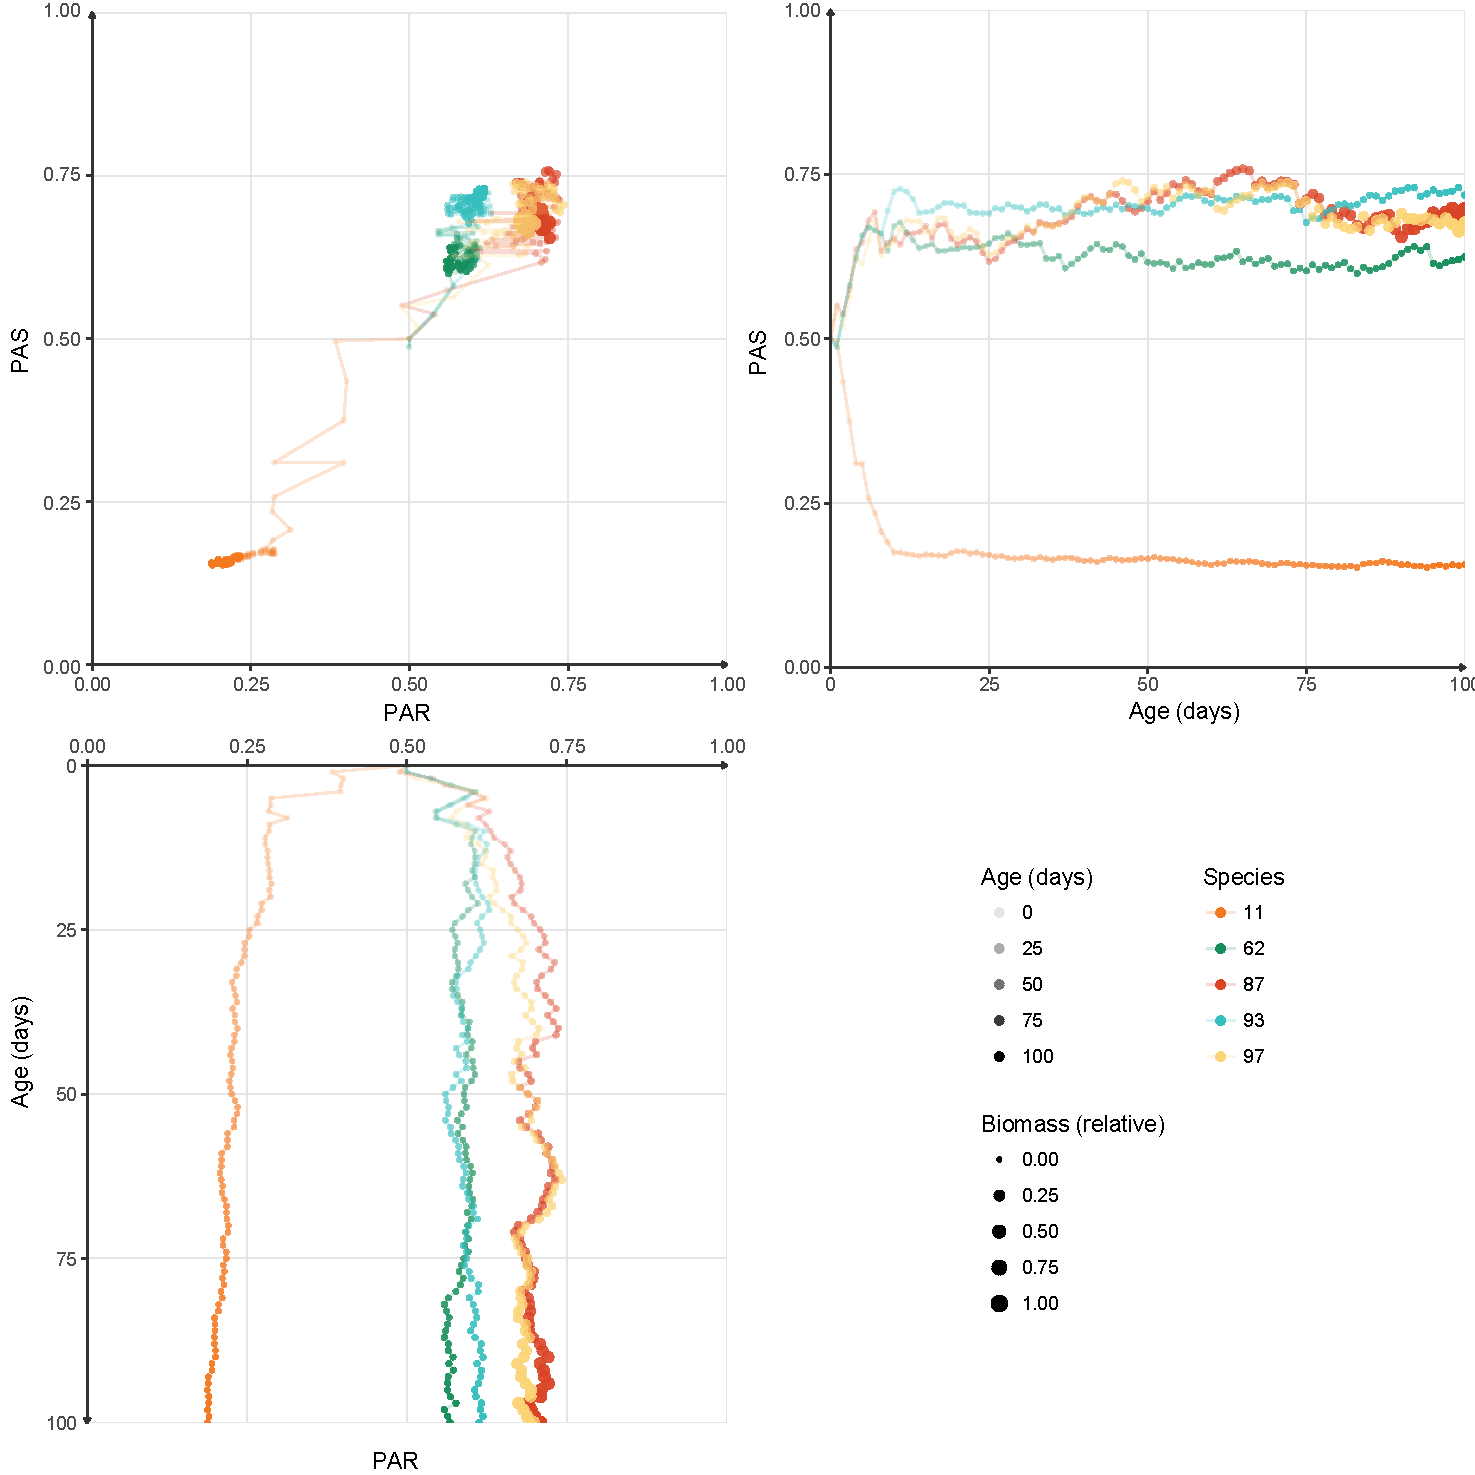
\includegraphics[width = \textwidth]{./2_PP/Figures/Individual/memory_effect.pdf}
\caption{Trajectories along time in the strategy space of 5 plants with different memories. After 10 days, all plants have converged toward the estimated optimum.}
\end{figure}

\paragraph{Memory and phenotype}

The kinetic of the phenotypic shift is first visualised for one parameter set on the two main phenotypic axis (proportion of active tissues in roots: PAR and proportion of active tissues in shoot: PAS). From the same starting point the five species show distinct rapid shift toward segregated subspace of the 2D strategy space. The equilibrium point is reached in approximately 10 days for all 5 species. Despite constant memory, variations are visible on both tissue allocation traits of roots and shoot. These variations lead to partial overlap but the five species are distinct on the 2D space.

The memory of resource availability is a strong enough driver to alter the default phenotype of a species. The effect of the two components of the memory (memory of water availability and memory of light availability) on the three main traits is explored through local regressions. The proportion of active tissues in roots increases to a plateau with increase in water availability memory (figure \ref{fig:w_ini_p_as_r}). This response pattern is consistent between all parameter sets, but the starting points and slopes may differ. The same pattern is observed between light availability memory and proportion of active tissues in roots (data not shown). The allocation convergence in the root is also influenced by the increase in light availability memory. An increase in the latter leads to a smooth increase in the former (see figure \ref{fig:l_ini_p_as_r}) with less drastic response than the water. This response is mirrored in shoot allocation response to increase in water availability memory (data not shown). Both organs react in symmetric ways to increases in resource availability. The RSR has a negative log response to water availability memory (positive in the case of light availability memory).

\begin{figure}\label{fig:w_ini_p_as_r}
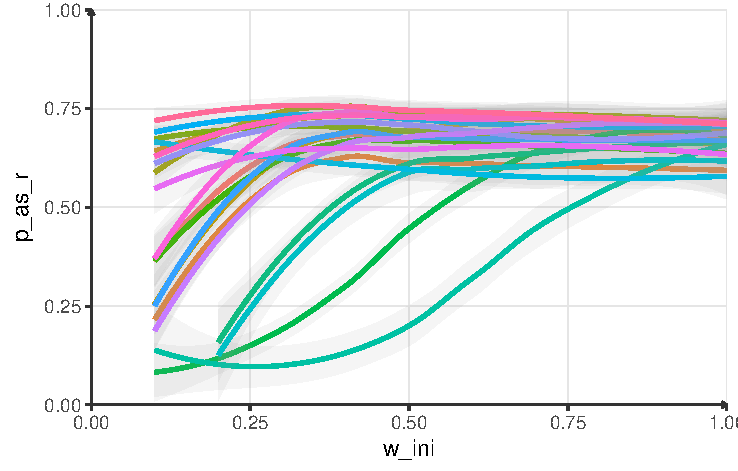
\includegraphics[width = \textwidth]{./2_PP/Figures/Individual/w_ini_p_as_r.pdf}
\caption{Effect of memory of water availability on proportion of active tissues in roots. \textit{Plastic-optimisation}. Each line correspond to a local regression fitted for all memory combinations for a given parameter set. Water availability memory is given in percentage of maximum exchange rate, absolute values may change between parameter sets.}
\end{figure}


\begin{figure}\label{fig:l_ini_p_as_r}
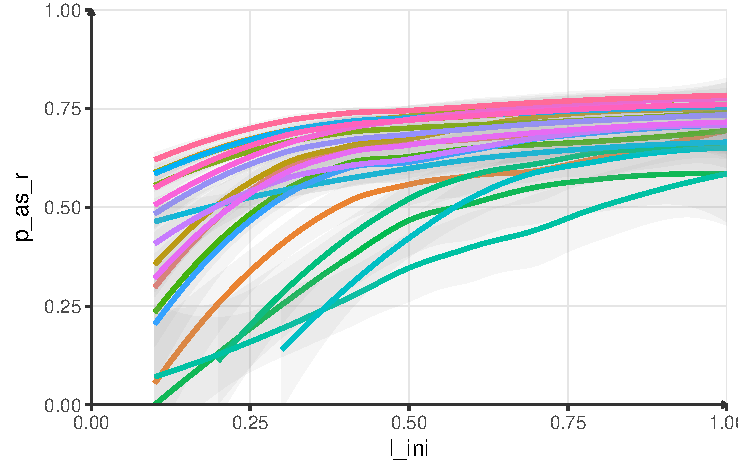
\includegraphics[width = \textwidth]{./2_PP/Figures/Individual/l_ini_p_as_r.pdf}
\caption{Effect of memory of water availability on proportion of active tissues in shoot. \textit{Plastic-optimisation}. Each line correspond to a local regression fitted for all memory combinations for a given parameter set. Light availability memory is given in percentage of maximum exchange rate, absolute values may change between parameter sets.}
\end{figure}

The combine effect of the two axis of plant resource availability memory is observed by plotting the phenotypes (on the 2D space of active tissue allocation) of four contrasting memories for all parameter sets (figure \ref{fig:memory_n_phenotype}). There is clear clustering of the four memory profiles, with some overlaps due to the fact that multiple parameter sets are plotted at the same time. The memory of low availability (\textcolor{myRed}{$\bullet$}) has a much larger distribution area than others, suggesting the relative instability of this profile within the "estimated net gain landscape". Memory of low availability for both resource drives plant toward very conservative strategies (need some values here) than other strategy. High expected availability of at least one resource increases allocation to active tissues to both organs. This confirms the positive effect of complementary resource (light for roots and water for shoot) of active tissue allocation in organs (see figure \ref{fig:l_ini_p_as_r}). Because of this, there is no highly unbalance phenotypes with high contrast between organ specific allocation emerging from the \textit{plastic-optimisation} allocation in \model. There is general coordination, but the balance between resource availability memories still impacts the position on the 2D, illustrated by the absence of overlap between low light - high water  (\textcolor{myBlue}{$\bullet$}) and high light - low water (\textcolor{myYellow}{$\bullet$}) phenotypes. In case of high resource availability and coordination, high investment in active tissues for both organ is achieved(\textcolor{myGreen}{$\bullet$}) and high light - high water), but the range of values is similar than for unbalanced memories(\textcolor{myBlue}{$\bullet$}) and high light - low water (\textcolor{myYellow}{$\bullet$}).

\begin{figure}\label{fig:memory_n_phenotype}
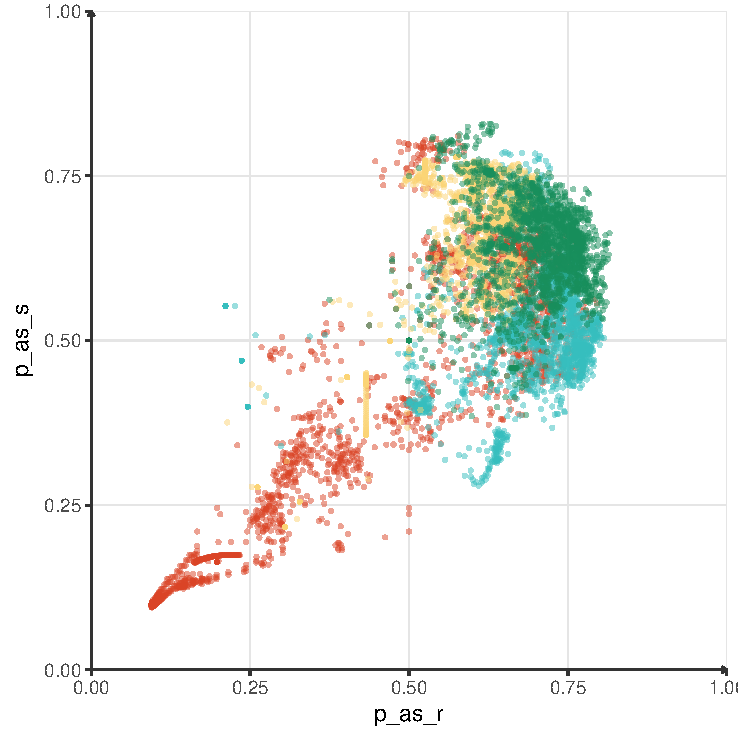
\includegraphics[width = \textwidth]{./2_PP/Figures/Individual/par_v_2D_points.pdf}
\caption{Impact of species memory on final phenotype in case of fully plastic allocation. \textit{Plastic-optimisation}. Each point corresponds to a plant phenotype for a memory syndrome for a given parameter set. Colours denote the memory syndromes.

\textcolor{myRed}{$\bullet$ low light - low water}, 

\textcolor{myYellow}{$\bullet$ HIGH light - low water},

\textcolor{myBlue}{$\bullet$ low light - HIGH water},

\textcolor{myGreen}{$\bullet$ HIGH light - HIGH water}.}
\end{figure}



\subsection{Discussion}
\paragraph{Allocation rules}

rapid convergence.\\

Cost and gains\\

Diversity of phenotypes\\

Crossed and symmetric influence: the respective efficiencies cannot be analysed independently.\\



\textbf{Allocation rules are extremely important as they reduce the phenotypic space explore. Without even considering plasticity. Need a good understanding of the performance within the phneotypic landscape. Plus there is a need for alignment between starting phenotype and endpoint. Will also affect how plasticity is driven.}

\paragraph{Fast-slow strategies}

... nothing here yet, the idea was to show that the "strategy" of the species conduce to slow and fast archetypes. Should be able to show that with some memory simulations.\\

But not equal distribution along the axis probably.


\textbf{Allocation trade-off allow for strategies from the fast-slow spectrum to arise, independently for shoot and root, in coherent framework. Potential effect of other strategy axis can be analysed alongside this trade-off, even if they affect composite traits like SLA or SRL.}

\paragraph{Memory and phenotypes}

 The symmetry and the curves shapes suggest that resource related organ is more sensitive and that "apparent" increase in resource availability promote more exploitative strategy. - what mechanism ?\\
 
It seems that there is greater concentration around high values of active tissues. This is consequence of net gain curves. Is this verified in other allocation rules ? Or is this an artefact ?
 
The role of memory highlight the expected problem of matching default phenotype with memory: little ontogeny effect (due to high growth and turn-over rates) and problem with distance based plasticity cost (would require a moving cost, instead of fixed reference cost).

For each parameter set the alpha shape of the volume could be drawn to have an idea on how parameters impact potential functional diversity. But no time here to test that.


\textbf{Memory is a strong enough driver to control plant organ strategy. The effect of overall activity should be studied too and considered if memory is used to determine the default phenotype.)}

Role of allocation rule and changes in traits, traits affect strategy and performance, memory lead to different phenotype/strategies (based on gain function), there is coordination, effect of complementary resource. Need to better understand allocation rule and optimum strategy, and convergence and diversity. 

\textbf{I REALLY NEED TO EXTEND THE CONCLUSIONS AND GO BEYOND MY OWN WORK. REFER MORE TO OTHER PEOPLE WORK ! ! !}

% ##################################################################################
\chapter{Individual performance, plasticity and variable conditions}\label{chapter:individual}

The previous section highlighted the ability of the model to model growth, but also the importance of species specific parameters. While the plasticity mechanism did not replicate to a full extend (stable and higher amplitude) the phenotypic changes between the  different conditions), there were some changes both in traits, and in growth leading to a higher selection rate. Considering the importance of species specific parameters and their potential impact on growth, these differences between plastic and non plastic allocation rules should be investigated in an extended manner. The specific roles of strategy and memory on the multiple components of plant growth need to be disentangled to draw better hypotheses on the role of phenotypic plastic on plant performance and coexistence. The role of resource availability on these mechanisms also needs to be interrogated. The effect of plasticity on coexistence can also be approached with respect to relative performances and contraction of the strategy space.

This chapter tends to answer these questions with simulations of individual plants with diverse strategies and under multiple allocation rules. To simplify the approach and focus on the interaction between species strategies and allocation algorithm, the plasticity will be model as discrete mechanism (tau = 0 for all plastic allocation algorithms).

\section{Individual performance: between strategy, memory and plasticity}\label{section:landscape}

This first subsection focuses on the link between the phenotype and the plant performance. The plasticity and allocation mechanisms can affect both the link between phenotype and performance and the distribution of the existing phenotypes.



\subsection{Method}

\paragraph{Parameter sets}
Because little differences are found between accepted parameter sets for the three main algorithms, parameter sets selected for the \textit{non plastic} algorithm are used for all algorithm. To reduce the number of simulations but have a measure of the genericity of the observed patterns, 20 parameter sets are selected among the accepted parameter sets for the \textit{non plastic} allocation algorithm. As mentioned in the previous section, the parameter sets have been selected for only one species-specific and therefore an additional step was used to filter out the parameter sets that could lead to high biomass values. For each parameter set, simulations of diverse phenotypes run for 100 days of 15 hours with favourable temperature conditions (20 \celsius) along resource availability gradient. The parameter sets are selected based on the maximum biomass of all simulated plants. One parameter set is randomly selected for each of the 20 brackets between 0 and 2 grams of total biomass.

\paragraph{Strategy space sampling}
To better understand what make a plant perform in the model, a multitude of phenotype needed to be tested. Tested phenotypes are distributed regularly along the three axis of the strategy space (proportion of active tissues in root, proportion of active tissues in shoot, proportion of roots) between extreme values (respectively (0.1, 0.99), (0.1, 0.99) and (0.1, 0.9)) for a total of 3375 combinations ($15^{3}$).  Because the RSR is defined by the memory, and in this set of simulation experiments the RSR is defined before, the species memory needs to be computed afterwards. There is an infinite number of couple of memory values that can match a given RSR. Also, the projection of conditions is sensitive to both memory and experienced conditions, therefore the choice of memory can affect the relative sensitivity of species to changes in external conditions and alter the model behaviour. Because the role of memory is not the focus here, and because there is much more focus on the role of the plasticity as a mechanism (as opposed as a strategy with various values of \texttt{tau}), the parameter \texttt{tau} is set to 0. This ensures that only the starting phenotype and the experienced conditions play a role in plant performance.

\paragraph{Simulation set-up}

For each phenotype a pot simulation is ran for 100 days of 15 hours under 4 millimetres rainfall and 120 Watt per square metres and per hour with the 4 main allocation algorithms (\textit{non plastic}, \textit{fixed-equilibrium}, \textit{fixed-optimisation} and \textit{plastic-optimisation}. Two resource levels are tested for each simulations. The low resource availability conditions correspond to a reduction by a factor 4 of resource influx, but the day length was conserved.

\paragraph{Projections}

To visualise the performance landscape (plant performance relative to biggest plant as function of its phenotype) the performance of best phenotypes are projected against the 3 plans that compose the phenotypic space. Such projections are preferred to 3D alternatives as they work better with static visualisation and when most of the space is occupied. Alternative axis are defined to facilitate the interpretation and description of the performance landscape: the organ strategy plane(PAR-PAS plane) can be transformed into strategy balance (difference between PAS and PAR) and "speed" (in sense of Reich \parencite{reich_world-wide_2014})(mean allocation to active tissues).

To study the potential effect of resource availability and or allocation mechanism on the link between strategy and performance, an aggregated measure is designed: the \textemph{gravity center} of the phenotypic space is defined as the average phenotype weighted by the relative performance of each phenotype. It can be defined with respect to the initial strategy, or to take into account the plasticity, to the final position in the phenotypic space. Shift of this gravity center within the projection space inform of translation of the performance landscape.

\subsection{Results}

\paragraph{Performance landscape}

\begin{figure}\label{fig:gravity_shift_resource}
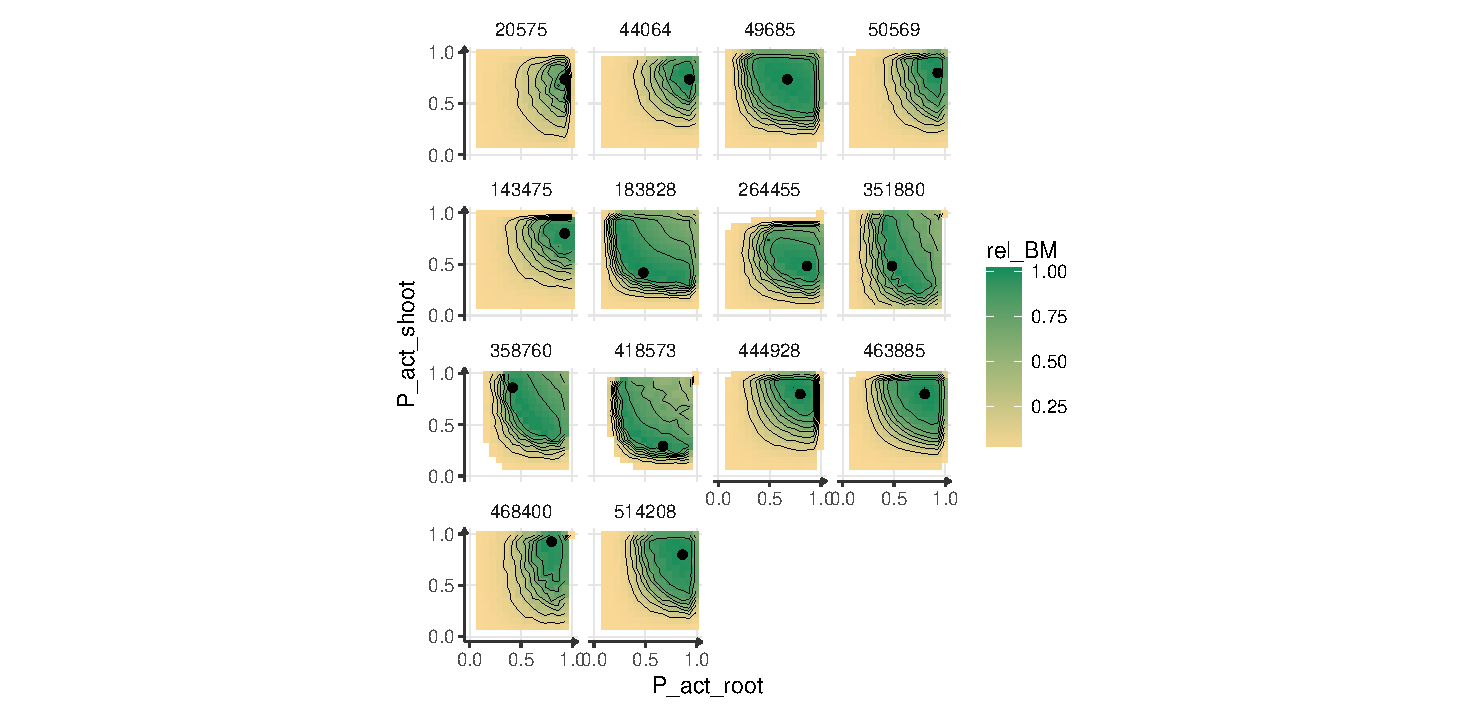
\includegraphics[width = \textwidth]{./2_PP/Figures/Landscape/ld_performance_PAR-PAS.pdf}
\caption{Projection of best phenotypes (varying RMF) on the 2D PAR-PAS plane for each parameter set. Points identify the optimums. \textit{Non plastic}.}
\end{figure}

 On the tissue allocation plan (proportion of active tissues in leaves and roots), the best performing phenotypes present a bean shape. This shape suggest that relative importance of organ efficiency is lower than other criterion such as equilibrium and overall performance (see section \ref{chapter:modelling_PP} paragraph \ref{subsection:match} for the discussion on the components of plant performance). On this plane, the lowest values of plant biomass are characterised by low values of active tissue allocation. 
 
Phenotypes with high active tissue allocation values tend to have lower growth values than phenotypes with similar values for one of the organ and lower value for the other organ. 

Projection of the best phenotypes over the three planes also gives information on the importance of the ignored variable on each plane. The greater the discrimination of the subset of best strategies on a given plane, the lower the importance of the ignored plane. The projection on PAR-RMF and PAS-RMF planes discriminate better phenotypes relatively to PAR-PAS plane, therefore the RMF is a more sensitive variable than the allocation factors to active tissues in organs.

If equilibrium is a driving mechanisms in plant performance, for any given strategy (PAR-PAS plan projection) the best phenotypes has a RMF values that guarantee the functional equilibrium. However, for each strategy there is a notable difference between the RMF of best phenotypes  and the RMF of phenotypes the closest to the equilibrium. This disparity is positively related to the strategy balance: best phenotypes with higher active allocation in shoot than root have lower allocation to roots than required for functional equilibrium. 

Higher resource: contraction of the landscape, toward faster species. Moving optimum and moving gravity center. Transition to optimum shifting and difference between allocation rules.


Biomass is relative to best performing non plastic plant (to remove the general parameter set effect on growth) and compare (within each condition) the effect of allocation algorithm. Plasticity lead to an increase of average relative biomass, especially full plasticity. However, few values above 1, in fixed conditions there is real additional value of plasticity compare to fixed allocation.\\

\paragraph{Optimum shifting}


A shift of gravity centres can be observed between the two resource levels in all plasticity algorithms. \textit{Non plastic} and \textit{fixed} algorithm show similar trends with an increase of proportion in active tissues in both organs. This change toward more exploitative tissues is consistent and is observable for all parameter sets but one. The \textit{plastic-optimisation} algorithm show drastically different responses of gravity center of phenotypes. There is little change in shoot proportion of active tissues, but a consistent reduction of active tissues in root system, and a reduction of root mass fraction (data not shown). These two responses indicates a net reduction of root activity in favour of shoot activity. Two things must be taken into consideration while looking at theese results: (1) the gravity center is computed from final position into the phenotypic space, not the starting position, (2) because \textit{plastic-optimisation} algorithm allows changes in traits that are represented (PAR and PAS), shifts along these axis can be driven by the plasticity mechanisms and not neceseraly only performance differences. Similar representation of the gravity center computed from the initial phenotype (not shown) shows similar response for the three first algorithms, and no apparent shift for the \textit{plastic-optimisation} plasticity.

\textit{Non plastic} and \textit{fixed} plasticities respond the same way to a shift in resource availability. However, we can note that the gravity centers have lower proportion of active tissues for \textit{fixed} allocation algorithm compared to the \textit{non plastic} one.

\begin{figure}\label{fig:gravity_shift_resource}
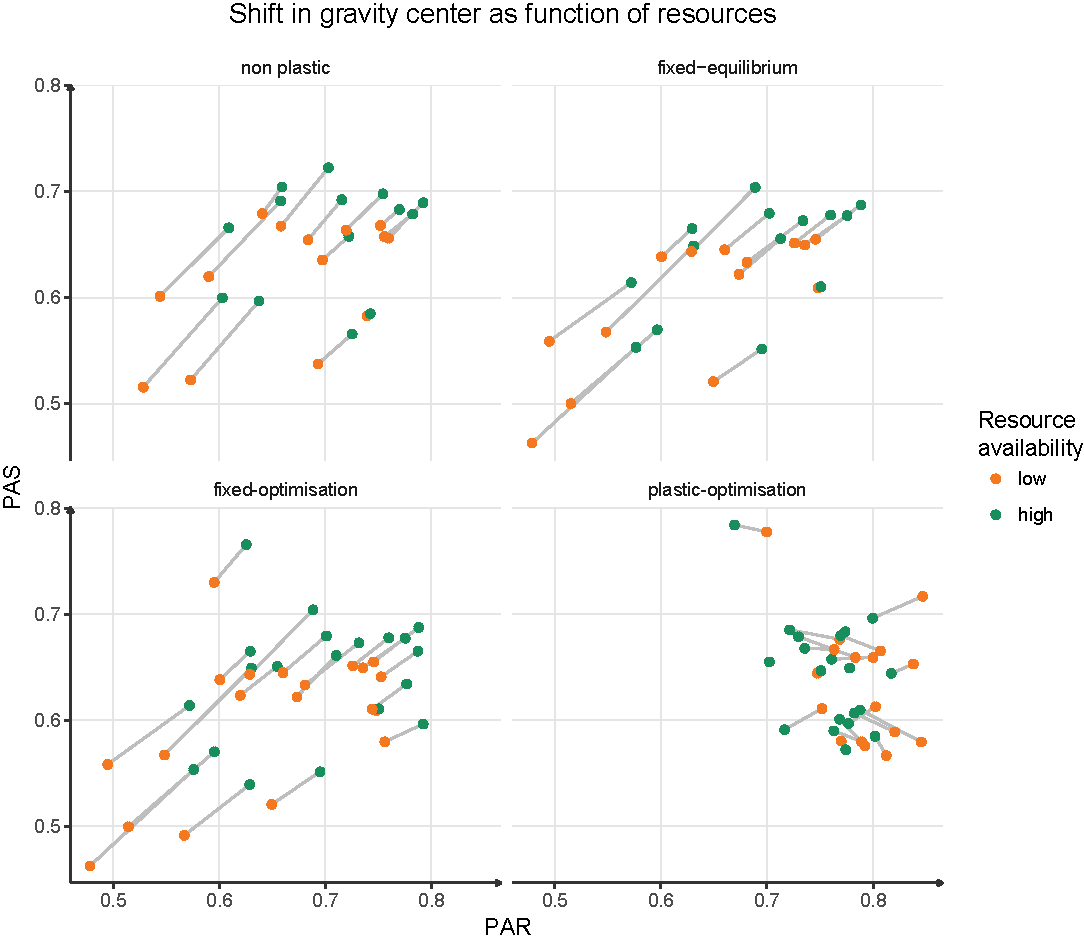
\includegraphics[width = \textwidth]{./2_PP/Figures/Landscape/ld_gravity_resourceall.pdf}
\caption{Shift on the 2D phenotypic space of the center of gravity as function of resource availability. The center of gravity is defined as the average phenotype weihted by the relative biomass, and characterises the performance landscape. \textit{Non plastic}.}
\end{figure}
%
%Shift due to plasticity -- timing only ?
%+ shift (not fully significant in high resource availability) toward more exploit shoot and less exploit root. What does that mean ? higher tissue efficiency authorized by less limiting water ?
%
%Where is the optimum ?  what makes an optimum ? Why is it important ? -- beter understand how plasticity works and can improve plant performance.
%
%What are the sensitive dimensions ? and why ? 
%
%then moving optimum and why ?
%
%Moving optimum 2D: why ?
%
%What is the plastic-optimisation doing ? Wrong phenotype ? Wrong projection ? Wrong strategy or wrong RMF ? 


\paragraph{Phenotypic convergence}
%\paragraph{Phenotypic space contraction}

\begin{figure}\label{fig:mean_BM_pl}
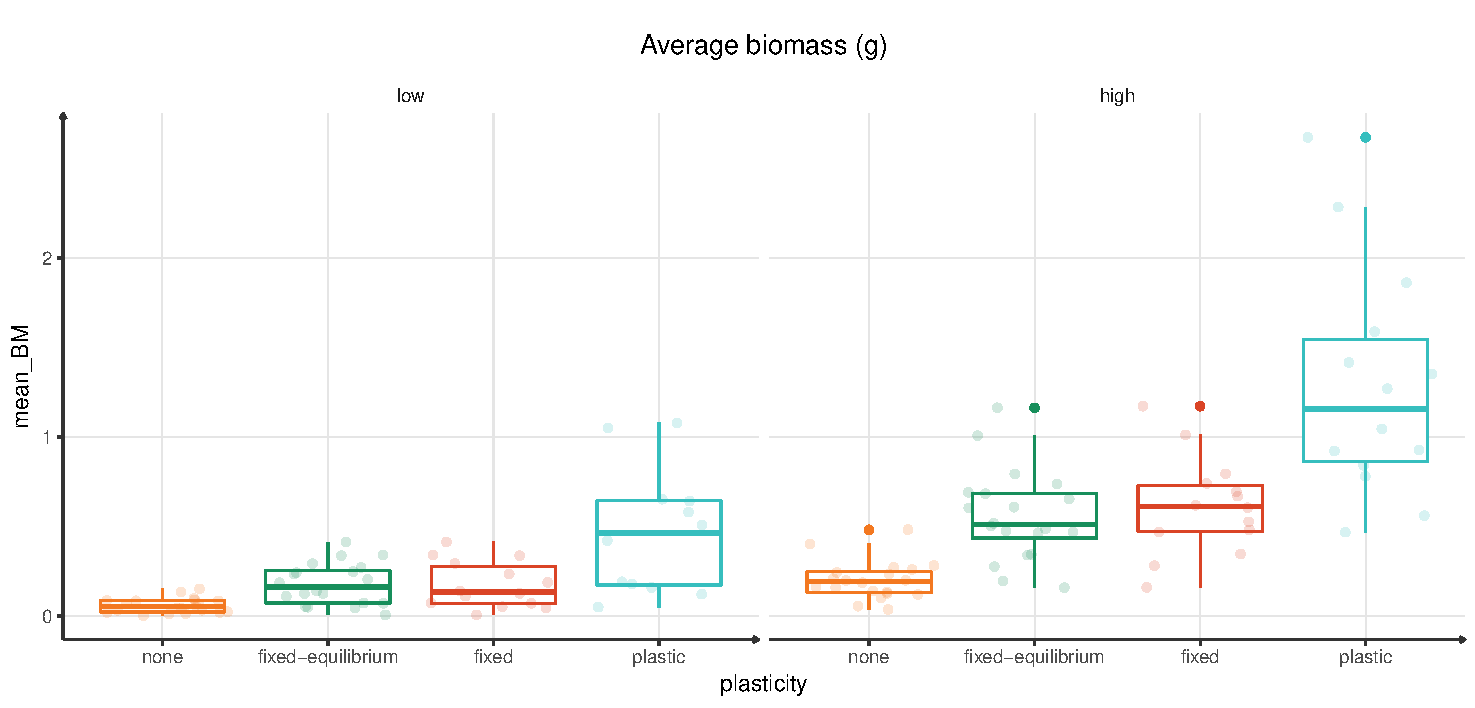
\includegraphics[width = \textwidth]{./2_PP/Figures/Landscape/plot_BM_allocation.pdf}
\caption{Mean relative biomass as function of allocation algorithm and resource level.}
\end{figure}

Shifts in optimum, is it because plasticity provide more efficient functioning supporting more exploitative strategies, or side result from convergence that do not contain the previous optimum ?

Convergence, relative species diversity and functional diversity.

\begin{figure}\label{fig:function_div}
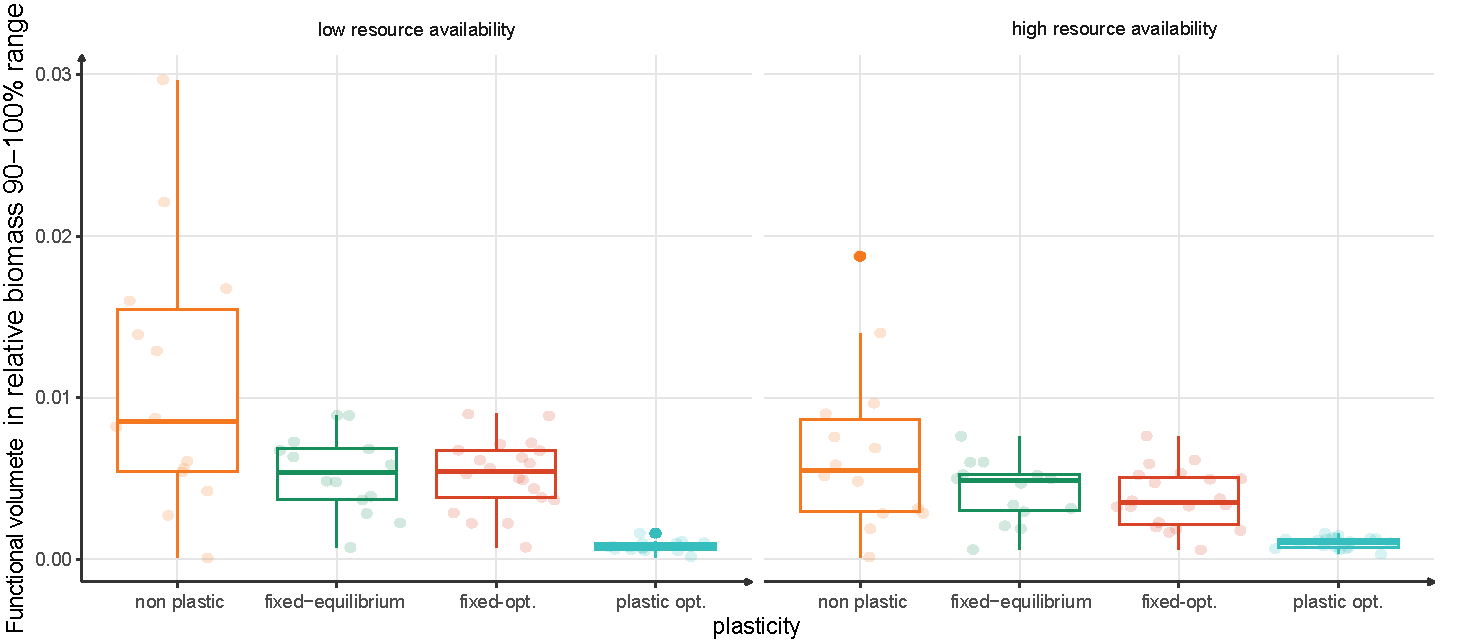
\includegraphics[width = \textwidth]{./2_PP/Figures/Landscape/plot_fdiv.pdf}
\caption{Functional diversity as function of allocation algorithm and resource level.}
\end{figure}




\subsection{Discussion}

\paragraph{Components of performance}

To understand how plasticity can play a role, it is important to understand what make a phenotype a good phenotype. In an other way it is important to understand what cost do a plant for being wrong.

\textemph{equilibrium}, overall \textemph{speed} and overall \textemph{efficiency}.\\
The main thing with equilibrium is the total resource use.

Better too fast than not fast enough.

Explain the memory stuff in previous section: low-low compared to low-high, the second one lead to overall higher productivity (lack of one resource compensated by higher allocation to the related organ) that can support more active tissues. 

The role of RMF: controlling variable, more sensitive than PAR and PAR but because bigger impact on balance: wide range on RMF values with similar performance: RMF value in itself is not that important: equilibrium is.

\paragraph{Convergence to subspace}

Phenotypic plasticity is often perceived with a species-centric perspective, that is to say, that plasticity is seen as variations in the species mean phenotype. However, in the context of community ecology, it is also interesting to try to see how it not only affect individual species but shape the community distribution in the strategy space. Plasticity relies on changes of default phenotypes toward "better" strategies in the context of the given conditions, therefore it implies that if it exists an optimum subspace (one strategy or an ensemble of strategies) species will converge toward this subspace, distorting the functional space. Environmental variations and plant interactions aside, in a constant environment the \textemph{performance landscape} is fixed. As a consequence the plasticity benefits to the plant in a static manner, that is to say, it is only a tool to reach a better phenotype where the plant stays in if conditions do not change. This can be related to spatial heterogeneity that would lead individuals from the same species to adopt different phenotype to acclimate to the particular conditions of their spatial situation. It is opposed to the perception of a more dynamic phenotypic plasticity as a tool for a given individual to cope with temporal variations in environmental conditions. These two aspects are further discussed in the following section, while the effects of the contraction of the phenotypic space are discussed now.

As explained before, plasticity can be seen at the scale of the species assembly \sidenote{here I draw a distinction between species assembly that refers to all present species, and community that refers to the interacting individuals of the present species. However, some interpretations can be translated to communities.} as a contraction of the phenotypic space of the species assembly. This contraction has two main effects: the reduction of potential functional diversity and a reduction of growth rate differences. There is here an emerging trade-off between the species diversity, supported by lower fitness differences, and functional diversity, reduced by the contraction of the phenotypic space. However, if the plasticity reduces greatly the potential functional diversity (volume of the whole phenotypic space without considering filtering based on relative fitness), the realised diversity (expressed as the functional diversity of the species within the 90\%-100\% maximum biomass range) is much less impacted because a large part of the phenotypic space (explaining the large potential functional diversity) has low growth rate in the given conditions. Nevertheless, the reduction of the diversity of expressed phenotypes is greater than it could ideally be. Indeed, in this scenario of "extreme" plasticity ($\tau = 0$) the convergence is important on plastic dimensions where it is not needed to have a significant increase in fitness (see conceptual figure \ref{fig:convergence}). Lower convergence on plastic dimension should lead to less compact phenotypic subspace while keeping relative fitness evenness. In the case of \textit{fixed-equilibrium} and \textit{fixed-optimisation} plasticity mechanisms, this effect is reduced by the sensitivity of the growth rate to the unique plastic dimension (see figure \ref{fig:plane_projections}). ... About \textit{plastic-optimisation} convergence...

Cost and distance, sensitivity to environmental cues as solutions to this problem. 

Because of high convergence of \textit{plastic-optimisation}, no improvment of maximum biomass, but the \textit{fixed} alternative thanks to convergence limited to one phenotypic dimension (RMF) higher biomass: either higher resolution, or improvement due to \textemph{dynamic plasticity}. The role of dynamic plasticity benefit is explore in temporal variation simulations in the following section.

\textemph{Convergence}

Somehow I need to talk about the cost of being wrong. Can be observe in the delta heatmap on delta strat and delta w-ini: in this case there is less impact of being wrong of memory if you're good with strategy, because your not in different conditions...\\

Potential effect on diversity: lower functional diversity, increase evenness. Leave highest fitness spot free. Why ? environmental cues or gain function ? Delta between projections ? \\

Anyway, being good is stable conditions may useless if cannot survive or keep gain in other conditions. >> look along gradient if best species keep their rank.\\


\paragraph{Plastic exhaustion}

\textit{Plastic-optimisation} algorithm is characterised by a high convergence of the species within the phenotypic space, high mean biomass but maximum biomass lower than best \textit{non plastic} phenotype, and high potential species diversity. The convergence is expected and explained by the fact that all three traits are plastic and all species (for a given resource level) experience similar conditions leading to the computation of the same optimum. The absence of plasticity cost limiting the convergence leads to a phenotype concentration toward this optimum. This convergence explains both the high potential species diversity, as all species have very similar growth rate, and the relatively high mean biomass because only few species did not survive or had very little growth rate.

The fact that this plasticity does not translates into higher maximum biomass is surprising, especially considering the fact that RMF plasticity improves maximum biomass (see figure \ref{fig:mean_BM_pl}). Lag in adaptation is often identified as a limit of plasticity \parencite{dewitt_costs_1998, van_kleunen_constraints_2005}, nevertheless, in a constant resource influx experiment, and considering the high phenotypic flexibility of plants in \model, this explanation is unlikely. Another problem highlighted with plasticity is its adaptiveness. Evolutionary speaking, it is hard to imagine the emergence and maintenance of a plasticity mechanism (in a given context) if it is no adaptive. Yet, such process could be maladaptive in a new context. Because plasticity is not emerging, but imposed by the simulation set up, its adaptiveness can be interrogated. Here adaptiveness do not refer to a reduction of fitness due to plasticity, but to the capacity of the plastic mechanism to define an optimum (or at least better) phenotype. Plasticity as implemented in model has no explicit bias and all mechanisms involved in plant growth are simulated by the allocation algorithm. The sampling of phenotypes is random and could be source of uncertainty, but it is uniform and no consistent drift is likely to emerge from the noise introduced by such sampling. The last aspect of plasticity that can affect the adaptiveness of plasticity is the estimation of conditions. The estimation of conditions is based on resource levels experienced by the plant and by definition are exact, therefore the problem lies in the projection of these conditions and how they translate into resource uptake.


\begin{figure}\label{fig:exchange_volume_projection}
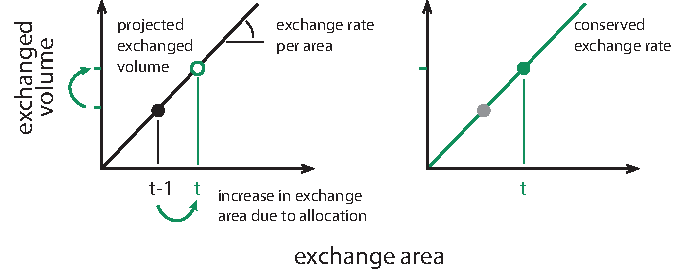
\includegraphics[width = \textwidth]{./2_PP/Figures/Concepts/exchange_volume_projection.pdf}
\caption{Projection of the water volume exchange after increase in exchange area at equilibrium and with no limitation.}
\end{figure}

In \model the resource availability is coded as an uptake rate per day and per unit of exchange area, and is computed as the resource uptake divided by the exchange area. This resource availability is supposed constant, and plants make the assumption that increasing their exchange area leads to a proportional increase in resource volume exchanged (see figure \ref{fig:exchange_volume_projection}).

\begin{figure}\label{fig:exhaustion}
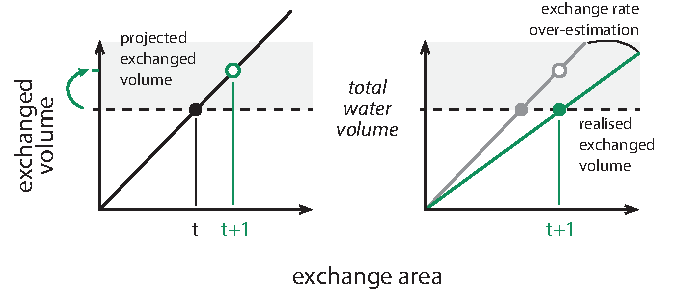
\includegraphics[width = \textwidth]{./2_PP/Figures/Concepts/exhaustion2.pdf}
\caption{Projection of the water volume exchange after increase in exchange area when total available water volume is limiting. The water volume exchanged cannot exceed the total available water volume, leading to a systematic over-estimation of water availability and offset between shoot and root activity.}
\end{figure}

However, in the case where a plant already absorbs all the available resource, then this assumption is not respected, and the uptake rate per area is lower than expected (see figure \ref{fig:exhaustion} right panel, realised exchanged volume does not match the projection because it cannot exceed the total volume of available water). This gap between perception and actual resource availability occurs because the plant is not able to perceive that the limitation cannot be compensated by a higher investment in the limiting organ. This behaviour explain a very high investment toward root and root active tissues in low resource conditions under \textit{plastic-optimisation} allocation (figure \ref{fig:gravity_shift_resource}). This gap\sidenote{this is different from a lag because it is not the result of slow changes in phenotype but comes from a default in the estimation of optimum phenotype.} is the cause of the \textemph{plastic exhaustion} phenomenon. Indeed, this constant over-estimation leads to constant discrepancy between the estimated optimum phenotype and the actual phenotype, and a larger allocation to root active tissues. This effect is particularly noticeable in the context of pot simulations where the water pool is limited. The absence of plasticity costs also favours such extreme behaviour. 

Despite this particular seemingly non-adaptive behaviour, the \textit{plastic-optimisation} algorithm is still interesting to study in community simulations. First, the presence of plasticity cost should limit such extreme behaviours. Second, in a context of competition in a larger environment, this aggressive search behaviour is likely to be an advantage against individual with less aggressive, or stable strategy. Finally, this mechanism emerges in constant influx conditions that allow growth, but its emergence should be reduced in variable environment where water shortage leads to reduced growth.

\textit{Plastic-optimisation} simulations expose this phenomenon with large effects, but it is probably present for simulations with other plastic allocations but with smaller effects. The difference in magnitude can be explained by a less effective growth in early stages of development for \textit{fixed} plasticities (when \textit{plastic-optimisation} is more efficient than fixed plasticities) that delay the time when the total volume is reached (time \textit{t} in figure \ref{fig:exhaustion}), and in average lower active tissue allocation in roots that leads to lower loss due to non-equilibrium.

\textbf{Plastic exhaustion is a specific limit of phenotypic plasticity as implemented in \model that relies on the assumption of constant exchange rate per exchange area. It has a large effect in the specific case of pot simulations. However, this phenomenon can be mitigated by plasticity cost linked to changes in traits, and can have adaptive value in a context of competition. Therefore, I argue that \textit{plastic-optimisation} algorithm  has low information value in the context of pot simulations with constant resource influx, but should still be studied in the context of community dynamics.}

\paragraph{Plasticity and information}

Limits exposed in this section and the previous can be explained by default of phenotypic plasticity mechanisms. Relies on assumptions that link partial information and strategy. There is no perfect informaiton (that would not even garantee best strategy). 

%make the link with limits of plasticity studies and the reliability of environmental cues. 

\paragraph{On functional diversity}

Can functional diversity be measured for plastic tratis: different effects on plastic and non plastic traits. 


\paragraph{Nuances around plasticity}
This analysis was conduced with drastic parameters of plasticity with plastic plants relying only on their perception of external conditions to develop their phenotype. The different results ... different directions and impact on potential diversity.

Also, some species may not benefit from plasticity, especially if it has a cost, while others can benefit a lot from plasticity.

The contrasting responses of the different algorithms highlight the importance of the allocation mechanism. However, the unique framework implemented in \model creates a variety of nuanced responses that are not all explored here. But, the continuous gradient of strategy between species relying on species memory only and species following their perception of external condition should be kept in mind during the interpretation of these results and following.
%
%\paragraph{On diversity}
%Effects on diversity.\\ I would put that aside for now
%
%The potential functional diversity is amplified by the fact that many phenotypes that are not viable in any condition but becomes viable thanks to static gain of plasticity. These species exist in the context of the simulation because there is no cost to plasticity. Because species are uniformly sampled in the 3D, a lot of them could not grow in a lot of conditions ?

\paragraph{Resource availability}

results from this part\\
As expected the resource availability and the resource balance are key components of the plant growth, to which the plant phenotype needs to match. Aside from the increase in biomass, an increase in "speed" of optimum phenotypes can result from higher resource availability. This observation is in agreement with empirical data that demonstrate higher SLA and faster physiology in favourable conditions. This aspect was less obvious in the response of species under \textit{plastic-optimisation} allocation that shifted more in term of balance and RMF. This may be due to a change in the relative balance between both resources as their availability (from the plant perspective) are linked to the global resource levels by non linear relationships.

The fact that plastic plants (for \textit{fixed} allocation algorithms) show shifts of optimum strategies toward more exploitative phenotypes, in addition to the \textit{non plastic} optimum shifts, in conditions of higher productivity demonstrate the importance of these strategies for plant growth. However, the extend of this effect of conditions on optimum phenotype is susceptible to vary along a gradient. Indeed, because of the non linearity of relationships between resource levels and exchanges rates, and between exchange rates and growth rates, the link between the optimum phenotype and a resource gradient is likely to be non linear itself. In addition, phenotypic plasticity might also change the sensitivity of the phenotype to the resource level.

Why we need to go for a gradient.

\paragraph{Greater level discussion}
? about what ? Community dynamics ? pp impact of these dynamics ? coexistence of species


\textbf{Subsection conclusion: bla bla bla}


% ##################################################################################
% ##################################################################################
% ##################################################################################


\section{Plasticity and variability of conditions}
Question I try to answer: (use of schematics ?)
The heterogeneity of conditions is an essential mechanism for plant coexistence. Plasticity is likely to alter the effect of this heterogeneity on plant coexistence and relative performance. The impact of plasticity on this relationship between spatial and temporal \textemph{heterogeneity} of resources (here limited to water) and strategy dominance is explored with the model \model.\\

Effect on optimum strategy: from previous conclusions and hypothesis to simulation method.\\
Then on diversity: how good strategies perform when it is plastic. Pool of species that exist in different conditions to get rid of the static effect.

\subsection{Method}

Because little coordination, and importance of below-ground resource acquisition (in the results, and in the context) and computational cost - only root strategies.

\paragraph{Simulation set-up}
For each of the 20 selected parameter sets, growth of 400 plants (20 PAR values between 0.25 and 0.95, and 20 memory values between 0.1 and 1) is simulated for 100 days in square pots of 12 centimetres deep and 90 centimetres wide (to avoid quick self-competition) in a temperature of 20 degrees celsius during the day of 15 hours, and 10 degrees during the night. Irradiance is set to the high values of 122 Watt per hour and per square metre. 

\paragraph{Spatial heterogeneity}
Spatial heterogeneity of water level is mimicked by a gradient of water influx. The growth of all 400 species described above are simulated for \textit{non plastic} and \textit{fixed-equilibrium} algorithm independently in separated simulations where the water influx is regularly sampled between 0.05 and 7 mm per day (20 values).

\paragraph{Temporal heterogeneity}
Similar set-up is used for temporal heterogeneity simulations. Because the range of water influx used in the previosus simulation is too wide, a lower value is chosen as the mean water influx. This value of 1.3mm per day corresponds to a point around which there is vairations in the optimum strategies for most parameter sets. It is also relatively close to average rainfalls in the Alps during summer. 

\subsection{Results: gradient of homogeneous precipitation conditions}

\paragraph{Optimum strategy}

Only look at the median of best strat. Gravity center lower for fixed-equilibrium, because of a few more species living.

The effect of allocation algorithm is observed on all species by plotting the position of the \textit{center of gravity} along the watering gradient that translates what part of the strategy spectrum (from conservative to exploitative) benefit from the simulation conditions. Along the gradient, conservative species exhibit higher growth than exploitative species with a median gravity center around ... \% of active tissues in roots for the \textit{non plastic} allocation algorithm, and ... \% for the \textit{fixed-equilibrium} plastic allocation. In the other end of the spectrum, for watering values above ... mm, the \textit{center of gravity} reaches a high point (median around ... \% of active tissues for both algorithms) demonstrating better performance of exploitative species in high resource availability conditions. Plastic (\textit{fixed-equilibrium} simulations show lower \textit{gravity center} in low resource availability than \textit{non plastic} counter-part. 
%
%
%\begin{figure}\label{fig:gradient_optimum_strat}
%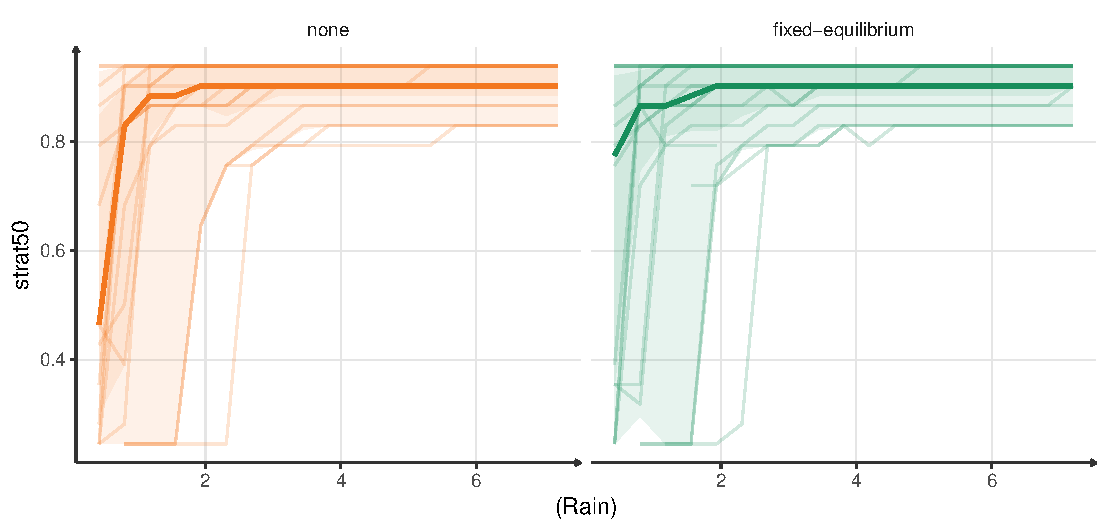
\includegraphics[width = \textwidth]{./2_PP/Figures/Rain/gradient_strat_trend.pdf}
%\caption{Median (dark line \textbf{-}) center of gravity of root strategy along the water treatment gradient for \textcolor{myOrange}{\textit{non plastic}} and \textcolor{myGreen}{\textit{fixed-equilibrium}} allocation algorithms. The color ribbons mark the band between the 25th and the 75th, and between 5th and 95th percentiles.} % Maybe I should change that so it is the 25th and 75th like for variable inputs.
%\end{figure}

As seen in the previous part, the shift in optimum can be caused by \textemph{static gain} but do not necessarily represent a change in optimum strategy. The effect of plasticity on the optimum strategy is tested along a precipitation gradient. Both algorithms are characterised by rapid shift from more conservative strategies in low water influx conditions toward high proportion of active tissues in root along the increasing rain gradient (figure \ref{fig:gradient_optimum_strat}).  There is not apparent differences between algorithms and the optimum is conserved along the gradient. There is a similar shift with an increase of optimum water availability memory for \textit{non plastic} algorithm.


\begin{figure}\label{fig:gradient_strat_trend}
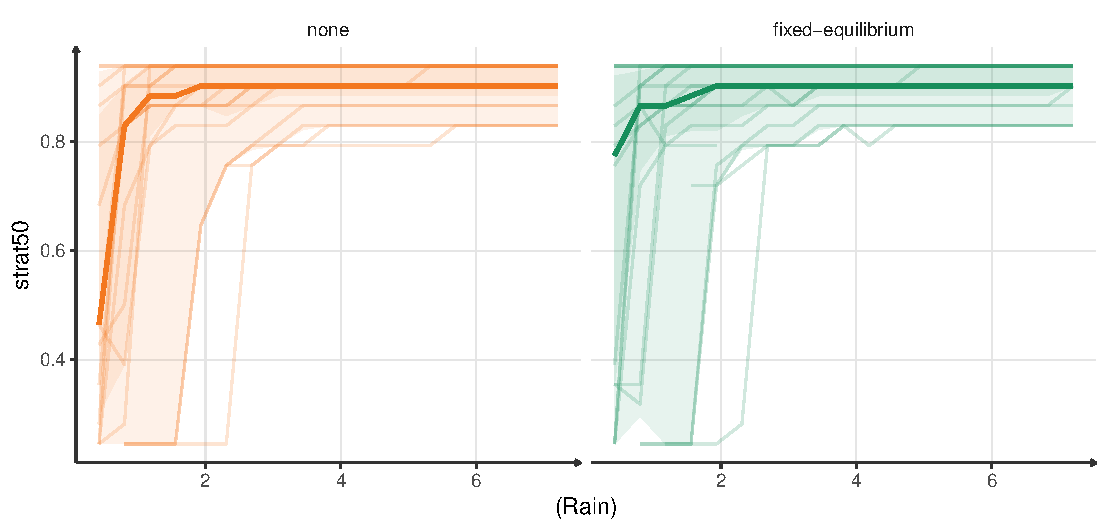
\includegraphics[width = \textwidth]{./2_PP/Figures/Rain/gradient_strat_trend.pdf}
\caption{Median (dark line \textbf{-}) optimum root strategy along the water treatment gradient for \textit{non plastic} and \textit{fixed-equilibrium} allocation algorithms. The light lines (-) correspond to the 20 independent parameter sets. The color ribbon marks the band between the 5th and 95th percentiles.} % Maybe I should change that so it is the 25th and 75th like for variable inputs.
\end{figure}


\paragraph{Bigger productivity?}

Strongly affect the potential overall productivity captured by cumulative biomass.


\begin{figure}\label{fig:total_BM}
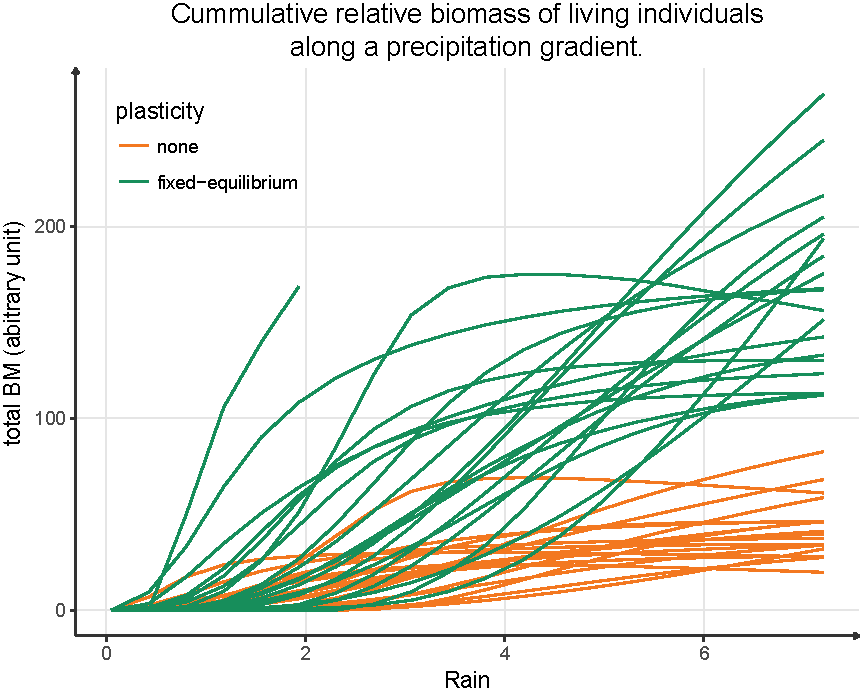
\includegraphics[width = \textwidth]{./2_PP/Figures/Rain/gradient_cumBM.pdf}
\caption[Total biomass along a precipitation gradient]{Total biomass of all individual along a precipitation gradient for all tested parameter sets. Colour distinguishes plasticity treatments: \textcolor{myOrange}{- \textit{non plastic}} \&  \textcolor{myGreen}{- \textit{fixed-equilibrium}}.} \end{figure}

 But, only marginaly (for a few parameter sets) increases the biomass of best species.

\begin{figure}\label{fig:maximum_BM}
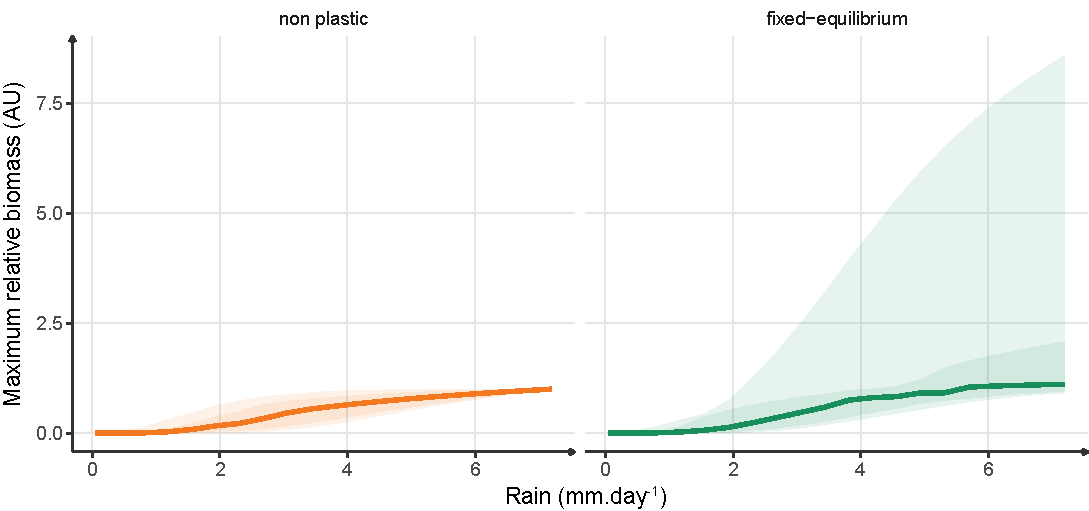
\includegraphics[width = \textwidth]{./2_PP/Figures/Rain/gradient_rel_BM_pl_trend.pdf}
\caption[Maximum biomass relative along a precipitation gradient]{Maximum biomass relative to the best performing plant in the most favourable condition for each parameter set, along a precipitation gradient.  Colour distinguishes plasticity treatments: \textcolor{myOrange}{- \textit{non plastic}} \&  \textcolor{myGreen}{- \textit{fixed-equilibrium}}.}
\end{figure}

That probably means more species reaching high performance levels.

\paragraph{What about diversity?}
Increase potential diversity as there is a contraction of the strategy space.

\begin{figure}\label{fig:species_richness_grad}
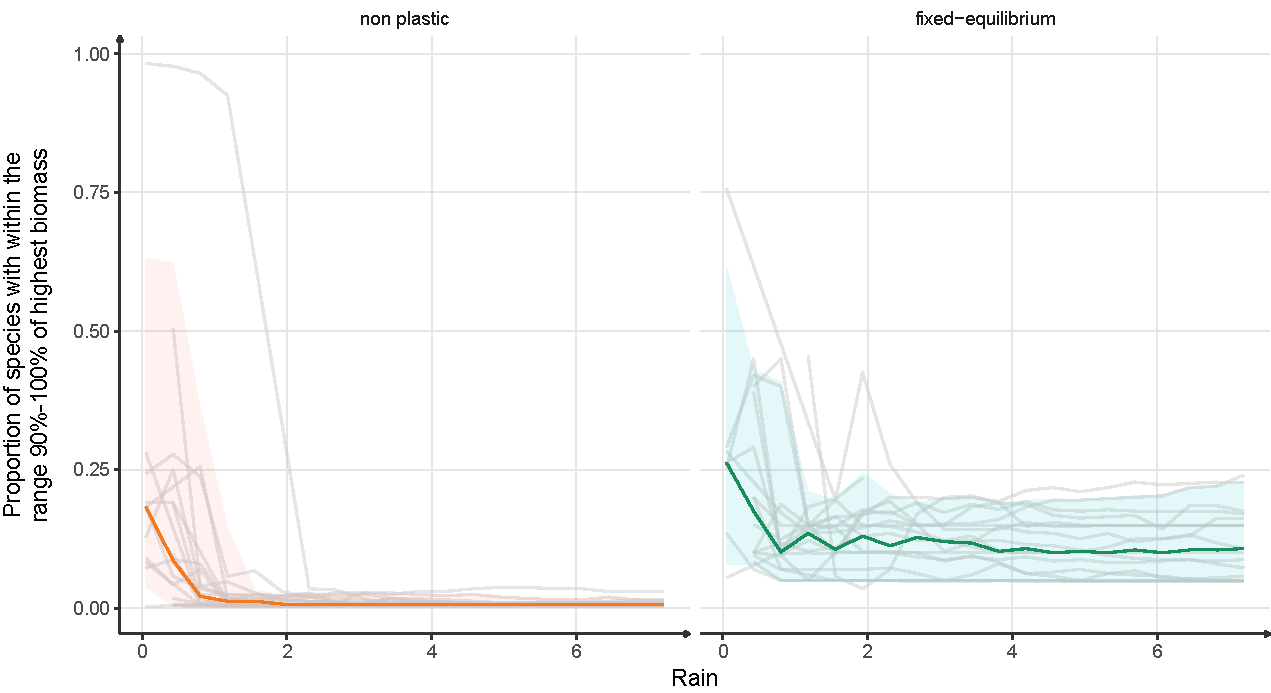
\includegraphics[width = \textwidth]{./2_PP/Figures/Rain/gradient_plot_spdiv10.pdf}
\caption[Species richness of the best performing species along a precipitation gradient]{Species richness of the species within the range 90\%-100\% of highest biomass for any given condition (parameter and precipitation) along a precipitation gradient.  Colour distinguishes plasticity treatments: \textcolor{myOrange}{- \textit{non plastic}} \&  \textcolor{myGreen}{- \textit{fixed-equilibrium}}.} \end{figure}


But does not change the functional diversity. 

\begin{figure}\label{fig:functional_div_grad}
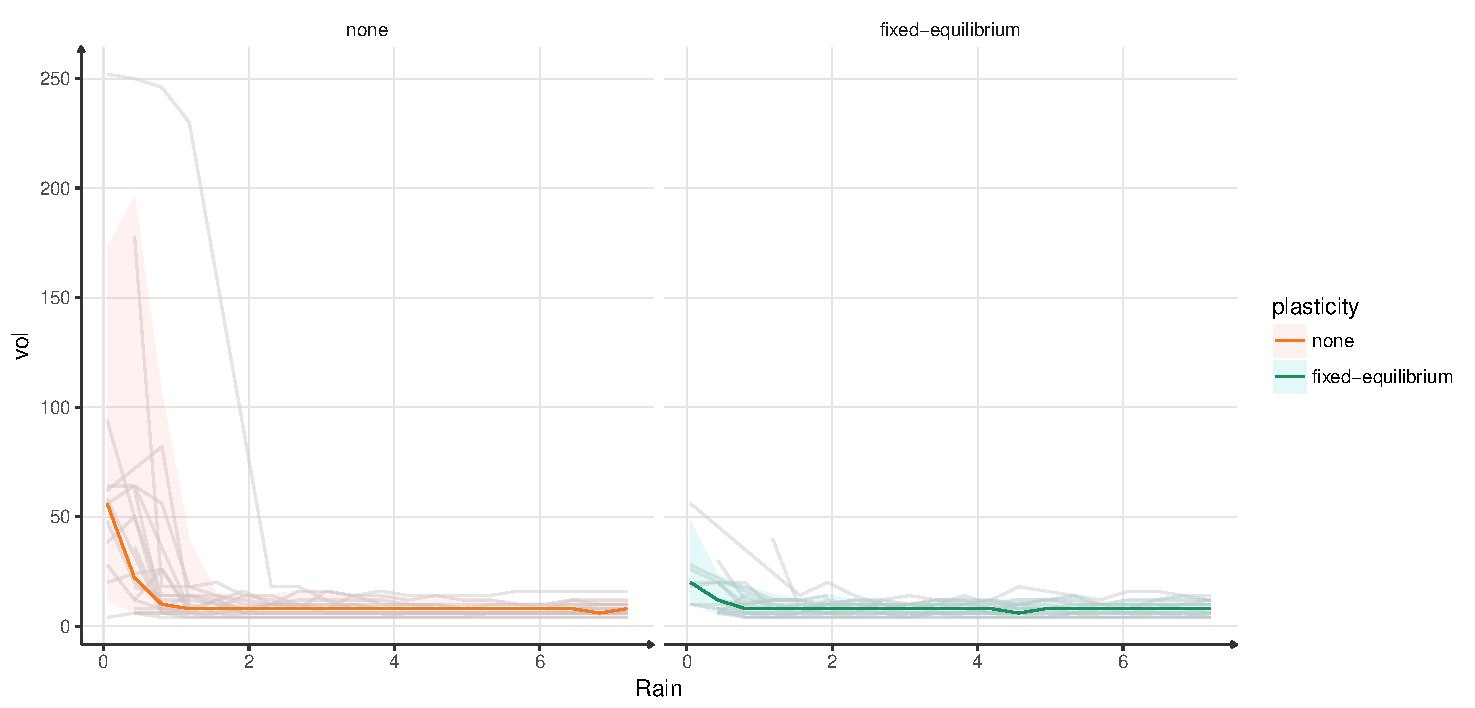
\includegraphics[width = \textwidth]{./2_PP/Figures/Rain/gradient_plot_fdiv10.pdf}
\caption[Functional diversity of the best performing species along a precipitation gradient]{Estimation of the functional volume occupied by the species within the range 90\%-100\% of highest biomass for any given condition (parameter and precipitation) along a precipitation gradient.  Colour distinguishes plasticity treatments: \textcolor{myOrange}{- \textit{non plastic}} \&  \textcolor{myGreen}{- \textit{fixed-equilibrium}}.} \end{figure}


\paragraph{Wider potential niches}

A lot of effects discussed here emerge because a lot of different memories (equivalently RMF values) are associated to each resource use strategy for roots (shoot active tissue allocation being fixed and shared by all species). Another way of looking at the effect of plasticity focuses on only species identified as the best in at least one of the rain conditions. This focus reduces the number of species to species selected along such gradient and allow to ignore species that would not be present anyway. This selection does not take into account any competitive mechanisms that could change the identity of the dominant species in a given condition. Nevertheless, information on how the relative performance of theses species can still be collected.



\begin{figure}\label{fig:gradient_ranking}
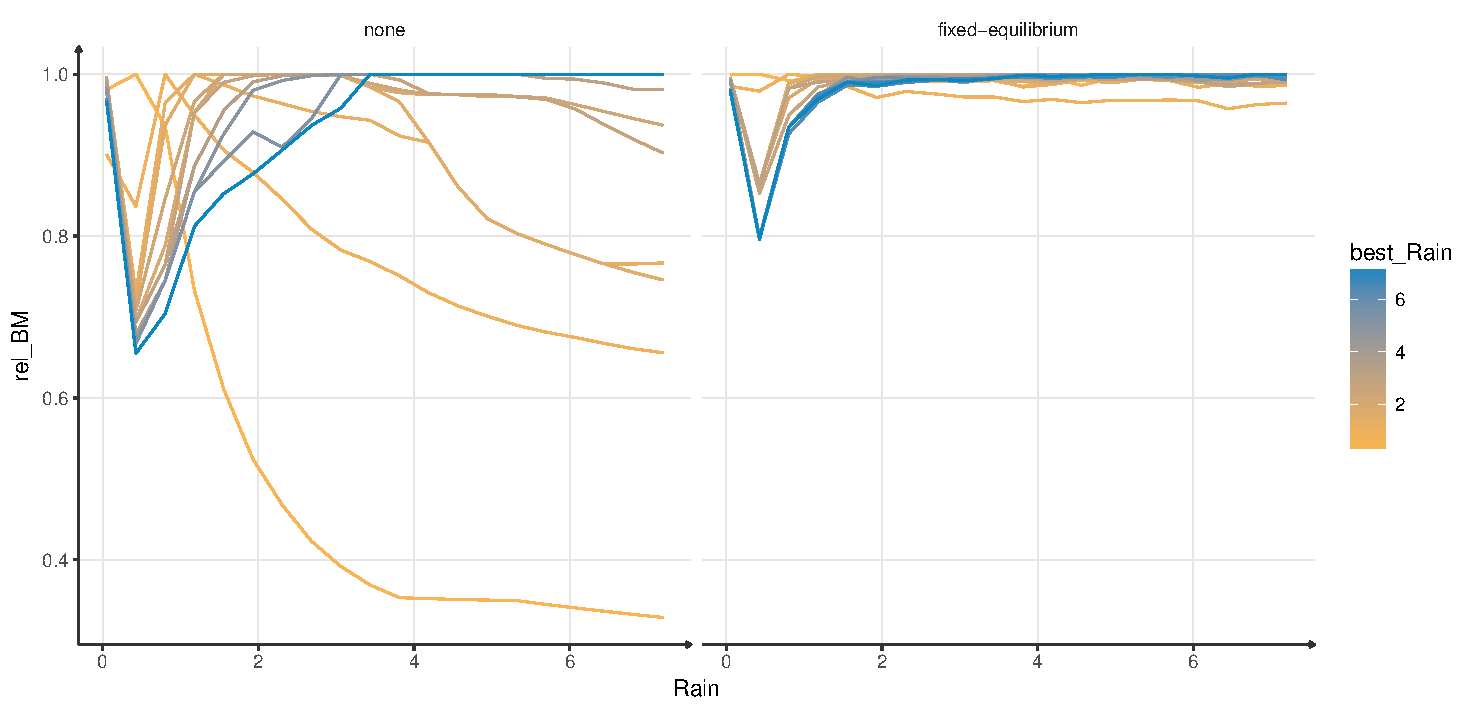
\includegraphics[width = \textwidth]{./2_PP/Figures/Rain/optimum_shifting_median.pdf}
\caption{Median relative performance of best phenotypes along a precipitation gradient for 20 parameter sets.}
\end{figure}

Changes in the niche ... but see:



\begin{figure*}\label{fig:gradient_ranges}
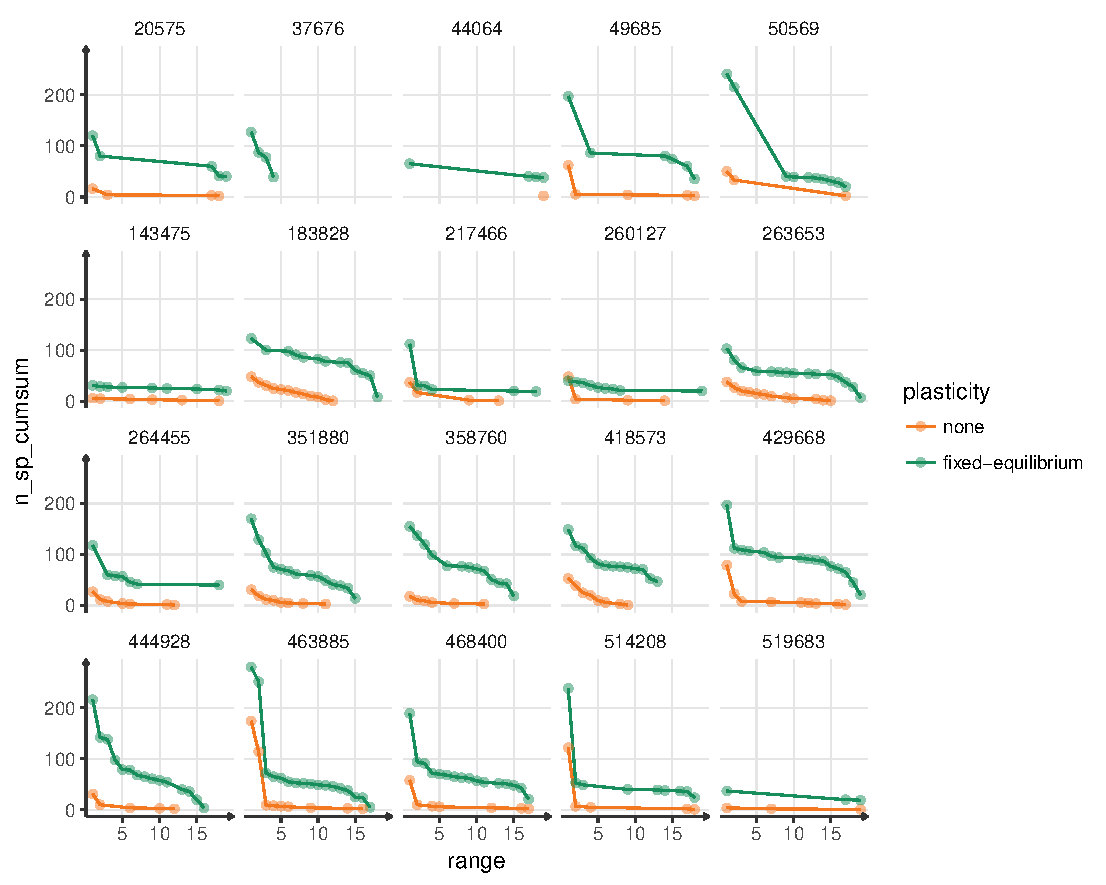
\includegraphics[width = \textwidth]{./2_PP/Figures/Rain/gradient_range_nb_sp.pdf}
\caption[Changes the dominance structure]{Changes in the dominance structure for the evaluated parameter sets. The dominance structure is illustrated by the cumulative number of species along diminnishing number of conditions where they are within the top 90\%-100\% range of highest biomass for any given condition. }
\end{figure*}




\subsection{Discussion: gradient of homogeneous conditions}

\paragraph{Strategy shift}
Along the watering gradient, the optimum strategy (active tissue allocation in roots) changes from conservative toward exploitative. This shift demonstrates that the trade-off between active and structural tissues allocation allows different strategy to dominate in constrasting conditions \parencite{}. This shift occurs for low values of the gradient and exploitative strategies are dominant over a large part of this gradient. This can be explained by high precipitation values disconnected from the precipitation values observed in nature. Also, the low resolution of the strategies (15 values for the proportion of active tissues in roots) limits the possible number of different dominant strategies along such gradient. 

\paragraph{Static and dynamic gain}
\paragraph{Who benefit from plasticity}

Gains from the plasticity can be distinguished between static and dynamic gains. The lower value of the \textit{center of gravity} in conditions of low water availability under \textit{fixed-e"quilibrium} algorithm seems to indicate that conservative strategies benefit from plastic allocation more than exploitative species. However, this effect is mostly due to static gain as the optimum strategy does not change. This 
effect is due to a growth landscape flatter than in better conditions (more species within the 90-100 \% of maximum growth, lower growth difference with best strategy) and asymmetric, that has two effects:
\begin{itemize}
\item it reduces the growth gain for species with strategy close to the optimum, but not at the equilibrium (figure \ref{fig:optimum_shift} panel A);
\item increases the potential gain (relative to less flat growth landscape) for species with strategies more conservative than the optimum (figure \ref{fig:optimum_shift} panel A).
\end{itemize}



\paragraph{Niche widening}

The phenotypic plasticity of the RMF leads to an important widening of the potential niche. This widening is, however, asymmetric because there is a transition of the limitations that define a species niche. Without plasticity, in a given homogeneous environment, the optimum phenotype is defined by both the adequate resource use and its balance. With costless plasticity in RMF, the balance is almost guaranteed and the resource use becomes the main limitation of a species niche. Conservative species are less efficient in high resource availability conditions, while exploitative species are more efficient, but this efficiency decreases quickly as the resource availability does not meet the levels required for these species to maintain high productivity.
 ... try to expend discussion on this idea.
 
 If cost are low, the effect is likely to reduce potential species diversity. An established species can, thanks to static gain, maintain relatively high growth rate in an habitat where the balance is different but the optimum strategies closed. This is particularly true for rich environment where the optimum strategy for roots is quite stable. The effect on coexistence is better illustrated with an example. Given two species, \textit{species a} and \textit{species b}, with optimum strategy (PAR) and RMF for two distinct conditions, respectivelly \textit{A} and \textit{B}, in a heterogeneous environment composed of majoritarely condition \textit{A} and minorly condition \textit{B}, ... where do I go with that ? ... 

%Reduce the structural role of spatial heterogeneity. Favour seed dispersal strategies. In high resource conditions, the resource levels do not matter much (non linearity of the optimum along gradient) but balance does, plasticity could reduce species richness, unless cost of plasticity. Unless not enough space to really be a niche (rare conditions): give opportunity to some species to extend their niche.

\paragraph{Fitness evenness}

Fitness evenness leads probably to greater competition has there is great overlap of potential niche. However, hard to tell what is the impact on competition and stabilizing effects. Probably negative: so hard to tell effect on coexistence.

\paragraph{What strategies benefit from plasticity?}

Who cares. The ones that are close to the optimum, unless there

\textbf{Mostly static gain, but even if there is gain, increases the potential niche of species that are settled. Bigger niche: favourable for conservative species of rare habitats.\\
Hard to tell anything on coexistence, except wider niches}



\subsection{Results: gradient of heterogeneous precipitation conditions}

Along the temporal heterogeneity (increasing negative slope of water influx) gradient the median biomass of the optimum phenotypes decreases under all allocation algorithms when the variability increases despite the same mean water influx. The amplitude of reduction varies with the allocation mechanism: \textit{non plastic} algorithm shows the largest decrease while \textit{fixed traits} algorithms show slower decrease. \textit{Plastic- optimisation} simulations have more constant performances with low initial performances in constant condition (between 5\% and 55\% on the \textit{non plastic} simulation), but they end with slightly better performances than \textit{non plastic} simulation for the extreme case of variation (two extreme regimes).


\begin{figure}\label{fig:variable_strategy}
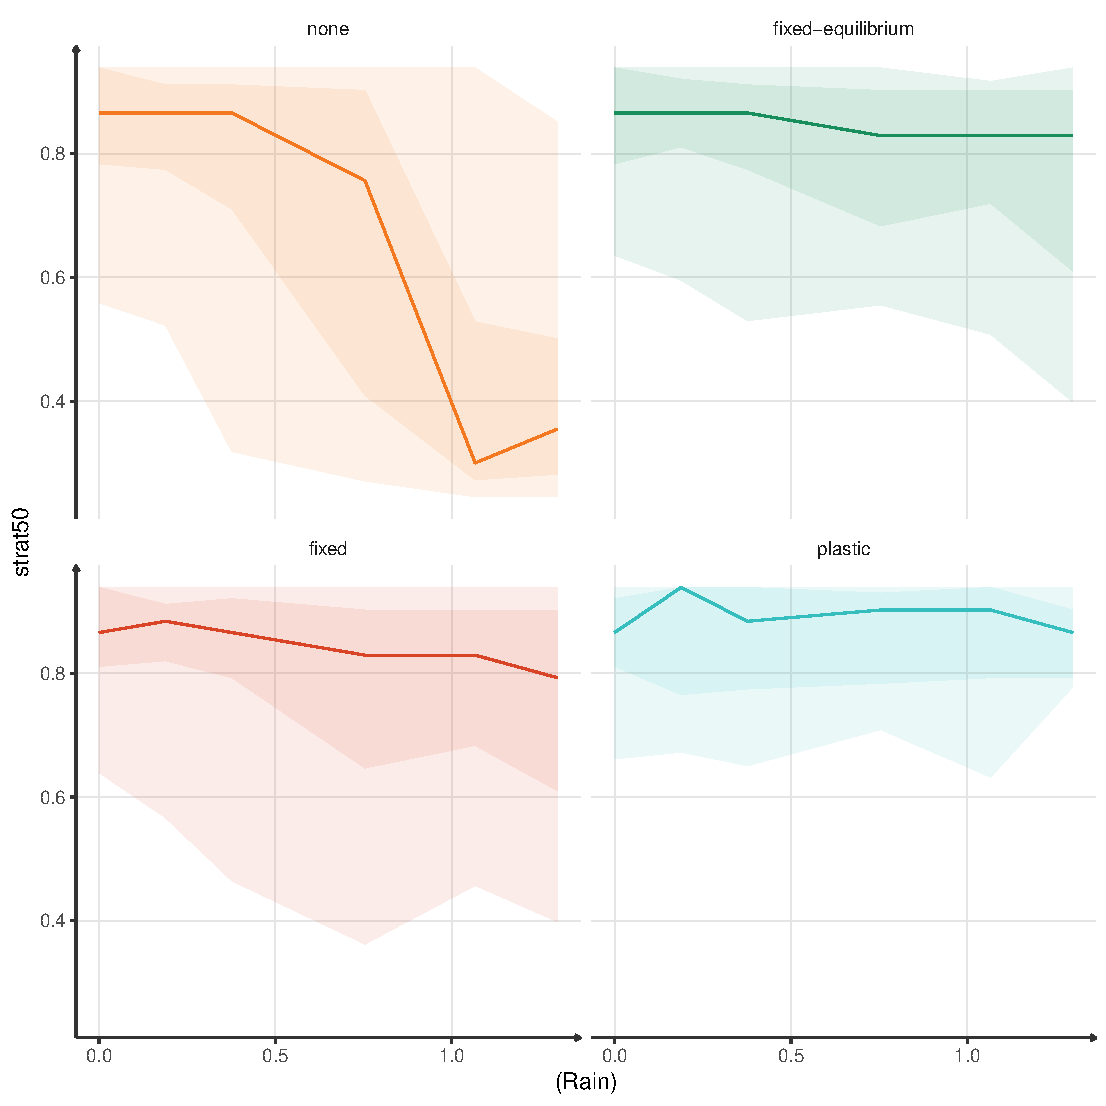
\includegraphics[width = \textwidth]{./2_PP/Figures/Variable/var_strat_trend.pdf}
\caption[Strategy shift along a gradient of resource variability]{Strategy shift of the best performing species along a gradient of resource variability for four plasticity treatment.}
\end{figure}

In addition to a reduction of biomass, the increasing slope of the water influx reduction lead to a shift of the optimum strategy in \textit{non plastic} simulations. This reduction of optimum toward more conservative strategies is offset in most of \textit{fixed-equilibrium} and \textit{fixed-optimisation} simulations. A reduction	(around 25\%) of the 5th and 25th percentiles of the optimum root strategy can be observed between the extreme conditions (constant flux and two distinct regimes) for these two algorithm. This shift in optimum strategy can better be observed on the plan of the proportion of active tissues in root (PAR) and root mass fraction (RMF) in figure \ref{fig:variable_trajectories} where all trajectories\sidenote{trajectory of the optimum, not of the species.} along the variability gradient are plotted. \textit{Non plastic} allocation trajectories by a linear shift toward more conservative strategies with higher allocation to roots, while \textit{fixed-equilibrium} and \textit{fixed-optimisation} trajectories are non linear and can be divided into two phases: (1) increase in RMF, (2) reduction of PAR. \textit{Plastic-optimisation} algorithm shows no consistent pattern in trajectories.


\begin{figure}\label{fig:variable_trajectories}
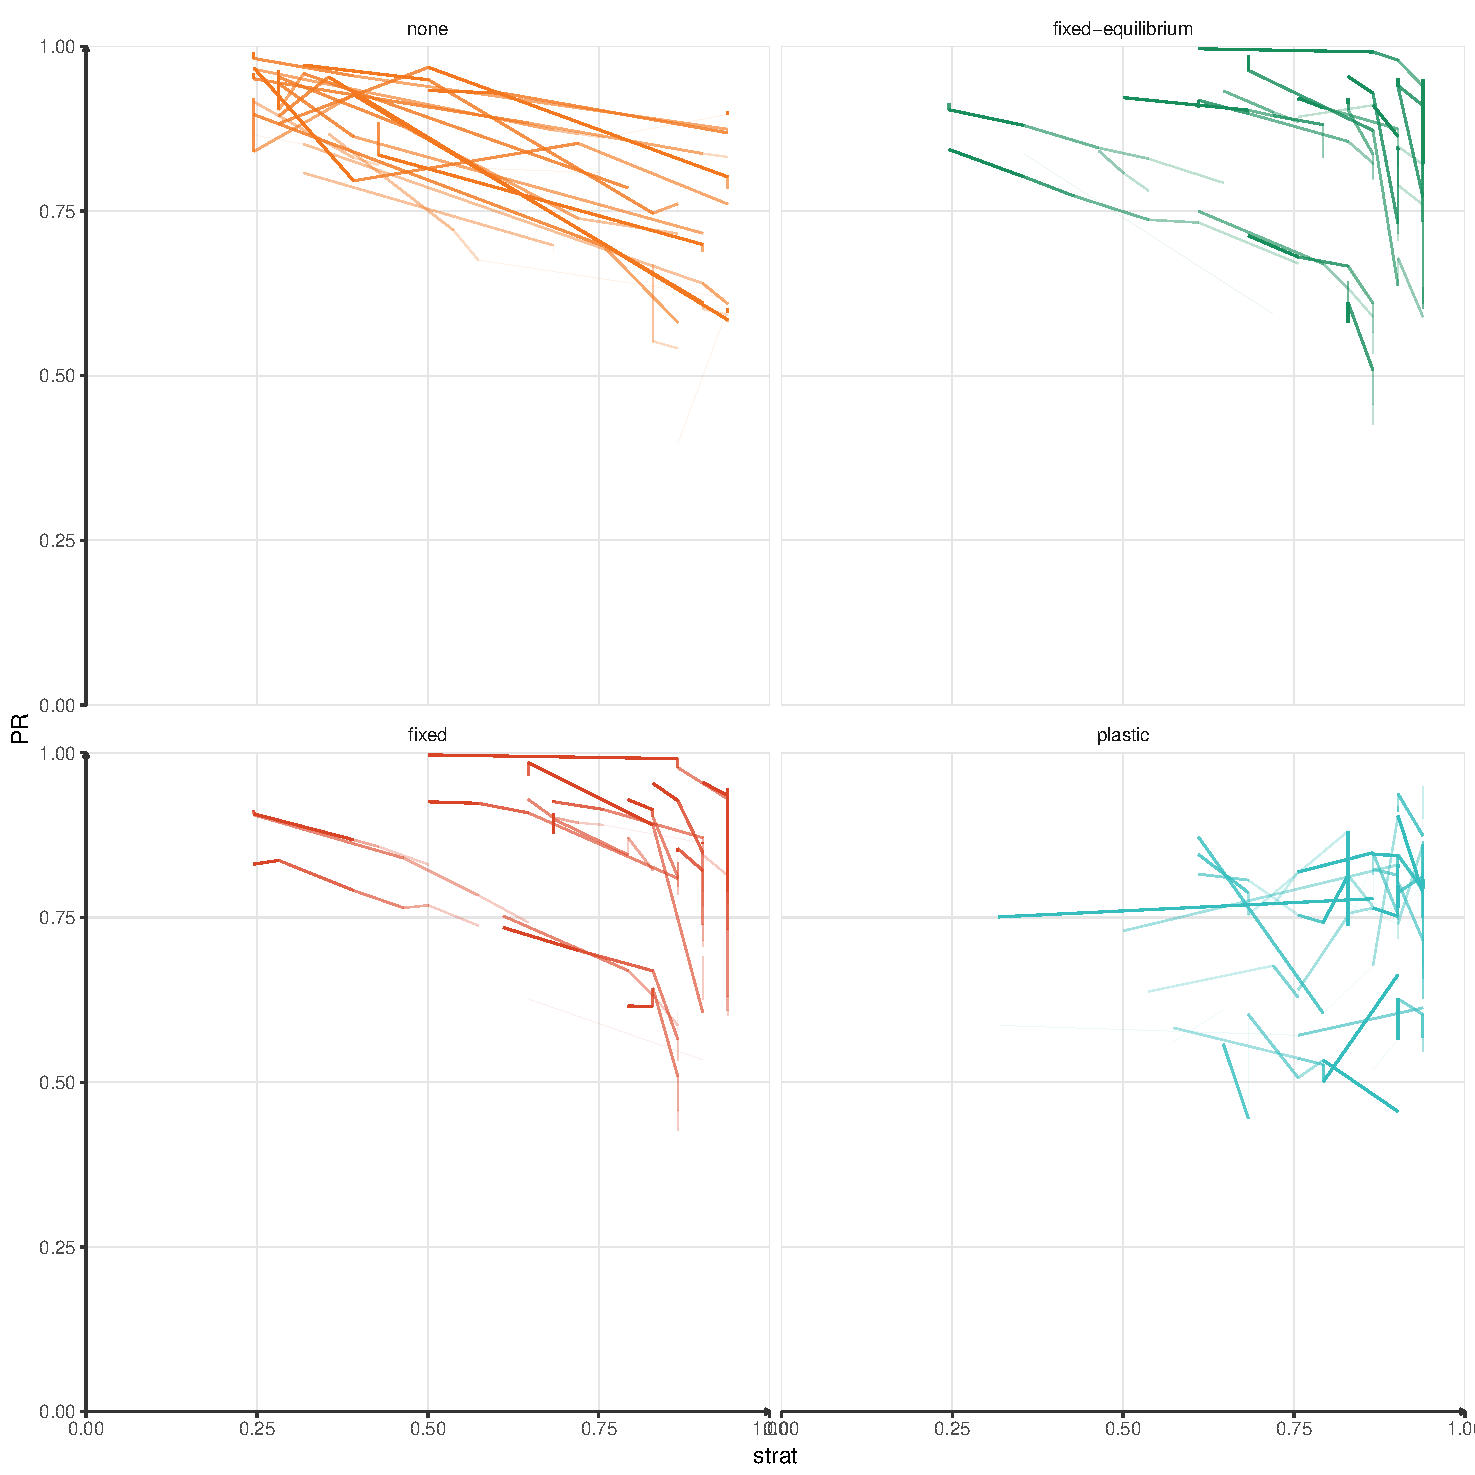
\includegraphics[width = \textwidth]{./2_PP/Figures/Variable/var_2D_strat_dyn.pdf}
\caption{Best phenotypes along water resource variability gradient. Thinner lighter lines indicate low water variability, while the thicker lines indicate strong temporal heterogeneity.}
\end{figure}

\paragraph{Diversity}

As previously seen, plasticity can affect diveristy in a drastic way, reducing the functional diversity by contracting the phenotypic space, but also increasing the potential species diversity by the same mechanism. The effect of static gain\sidenote{refers to the gain due to convergence toward a good static phenotype and no temporal changes.} and dynamic gain must be disentangle. The 


\begin{figure}\label{fig:variable}
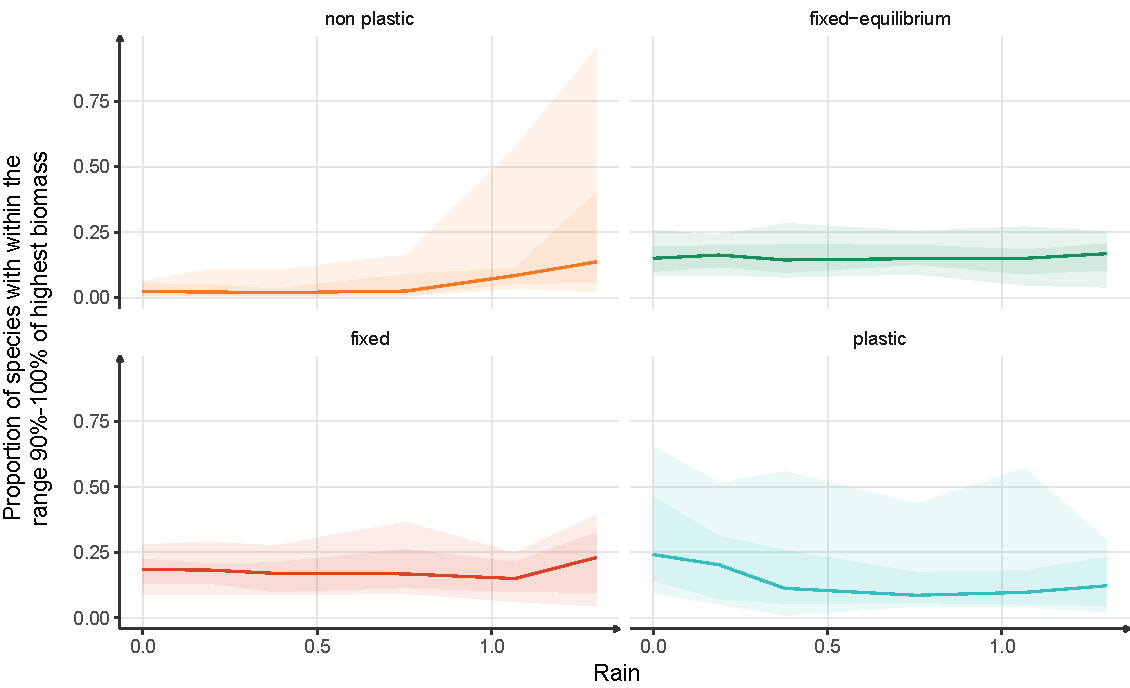
\includegraphics[width = \textwidth]{./2_PP/Figures/Variable/var_spdiv_trend.pdf}
\caption[Species richness of the best performing species along a water resource variability gradient]{Species richness of the species within the range 90\%-100\% of highest biomass for any given condition (parameter and precipitation) along a water resource variability gradient.  Colour distinguishes plasticity treatments: \textcolor{myOrange}{- \textit{non plastic}} \&  \textcolor{myGreen}{- \textit{fixed-equilibrium}}.}
\end{figure}


Changes in optimum, but does it affect eveness ? Same pattern as before with tehe trade-off between species and functional diversity. What happen if you filter down stuff ?





\subsection{Discussion: gradient of temporal variations}


\paragraph{Improvement in variable conditions}
Plasticity has a a positive effect on exploitative strategies in low resource availability conditions. As said earlier in the document, plant performance depends on multiple things: effectiveness of organs, global resource usage and equilibrium. 
% Here talk about the spatail heterogeneity:
If plasticity improve the performance of the exploitative species, it is unlikely to be because of the contraction of the space since it is the optimum only that is looked at. Also means it is probably dynamic gain, it the filter was static, plasticity shouldn't have change much. And there is gain, even in the high end of the gradient where the optimum does not move, saying that the optimum is fairly conserved despite increase in resource (but low resolution of the strategy space, and match the function). 

% From theere, talk about the variable rain input.
Change in optimum strategy can be explained by: an assymmetry in efficiency (better a but more conservative in exploitative favourable conditions than exploitative in conservative favourable conditions) or an assymetry in inbalance cost (better be inbalanced when conservative than when exploitative). The first option is not consistent with previous results (see subsection \ref{section:landscape}, figures ...) that show higher fitness for species more exploitative than the optimum, compared to species more conservative. In the other hand, following results show positive effect of functional equilibrium over conservative strategies. Nevertheless, this effect certainly results from an artefact and the contraction of the phenotypic space not in favour of exploitative strategies. The sensitivity of exploitative strategies to low conditions is visible in figure \ref{fig:gradient_optimum_strat}

Shift of RMF then strategy explain quite well that the equilibrium is more important than the resource usage and the organ efficiency. How does that inform us on the real world ?

 - potentially reduces the meta community diversity if spatial heterogeneity has a less drastic effect on strategic dominance. - talk about that in diversity part

/!\\ may come from a lack of coordination with shoot. Since shoot activity is suppose to be relatively high. == might not have besn a good choice to look only at root strategy. But, since there is adjustment of RMF that allow to maintain equilibrium and resource usage, it should be fine to interpret these results.

\textbf{Phenotypic plasticity give exploitative species an advantage in variable conditions because their growth rate rely more on productivity and therefore equilibrium than conservative species. }

%\paragraph{Heterogeneity of response}
%
%Kichenin (different response to gradient) Doesn't work in this framework: Not so sure about that: depending on your initial memory plants show directional changes toward one phenotype. Yeah, but they should have converged for other conditions too... So, it doesn't work. Might be explained by:
%\begin{itemize}
%\item different conditions: because heterogeneity and habitat selection, or changes in competition hierarchy;
%\item different ways to tackle changes on one dimensions;
%\item different weights between mechanisms impacting composite traits, because of the different traits.
%\end{itemize}




\textbf{The phenotypic plasticity implemented in \model improve the relative performance of multiple strategies by concentrating the plant toward a subspace of higher performance for most of plants. Convergence to a smaller subspace can be assimilated to reduction in phenotypic diversity, but it reduce performance heterogeneity and should favour local plant diversity. However, this effect should be limited by plasticity cost. Indeed, if the growth gain due to plasticity is only static, any species with a fixed phenotype closer to the optimum than the focus species has a better growth rate and exclude the focus species.
. a few words on dynamics... Meta-community diversity is however reduces by the reduction of potential axis for niche differentiation. Plasticity costs and limits should play major role in the balance between these mechanisms. Community level simulations are needed to further understand the cumulative role of competition, spatial and temporal variability and plasticity costs on phenotypic plasticity influence on plant community dynamics.}


\section{From model behaviour to competition and coexistence in the real world}

\subsection{Plasticity: new functional diversity}

functional diversity of plastic traits? Should them be excluded?

Impact of traits, and abundances: the need to account for it!

May still be useful especially for invasion, and works well despite low flexibility (see \parencite{forsman_rethinking_2014}. May allow more diversity if some correlations with other non plastic traits.	

\subsection{Plasticity as a strategy: cost and correlations}

\paragraph{Who benefit from plasticity?}

\paragraph{Cost of plasticity}

and limits ? what about exhaustion

\paragraph{Plasticity as a strategy}
One of the argument to say this is new, however not really explored, neither with plasticity cost perspectives (a bit with plasticity limits) or with tau. However, used extreme cases: give better understanding and necessary before finer analysis. Still, there are hypothesis on the effect on diversity and the role in phenotypic stability (attention: isn't it just because the formulation of projection is wrong that we can make these conclusions ?).



\subsection{Plasticity and competition: changes in interactions}

\paragraph{Extended interpretations}
What about the continuous $\tau$ gradient ?\\

What about interactions and cycles ? Little has been discussed on the dynamic of the resource and how it could affect coexistence. Imagine that with cycle, reproduction timing has an importance here...


plasticity will change: performance, sensitivity and impact of the resource.

%\section{From individual response to community dynamics}

% Use these notes to extend the discussion and add some outlooks
%
%\section{Niche response}
%
%
%Obj1: understand how resource use mechanisms and allocation algorithms shape the environmental potential niche in the context of the model.\\
%H1: strategy and memory affect niche in two ways if we suppose they are independent: shape and position. Strategy mostly affect shape (width and height) while memory (and so root:shoot ratio) affect mostly position.\\
%H1': there is strong link between strategy and memory in the case of optimisation allocation that increase niche height and might reduce its width.\\
%Obj2: understand the role of plasticity on the niche and if the effect in the same for all strategies/memories.\\
%H2: the plasticity increase niche width but not height (as phenotype is optimum at the center of the niche where memory match the resource availability).
%
%Stability and efficiency trade-off. Niche heigh and width and relationship with the strategy. How does plasticity affect that ? Does it increase the height and widen niches ? What does that mean for coexistence ?\\
%Hopefully higher niche would go with unstable niche.
%%
%%\section{Transitivity and competition}
%%1 vs 1 interactions\\
%%Is the resource competition transitive ? How does niche widening impact that, does plasticty change competition interaction. Is it related to the trait distance ? (don't think so)
